\newif\ifen
\newif\ifes
\newif\iffr
\newcommand{\fr}[1]{\iffr#1 \fi}
\newcommand{\En}[1]{\ifen#1\fi}
\newcommand{\Es}[1]{\ifes#1\fi}
\estrue
\documentclass[shownotes,aspectratio=169]{beamer}

\usepackage{siunitx}
\input{../../auxiliar/tex/diapo_encabezado.tex}
% tikzlibrary.code.tex
%
% Copyright 2010-2011 by Laura Dietz
% Copyright 2012 by Jaakko Luttinen
%
% This file may be distributed and/or modified
%
% 1. under the LaTeX Project Public License and/or
% 2. under the GNU General Public License.
%
% See the files LICENSE_LPPL and LICENSE_GPL for more details.

% Load other libraries
\usetikzlibrary{shapes}
\usetikzlibrary{fit}
\usetikzlibrary{chains}
\usetikzlibrary{arrows}

% Latent node
\tikzstyle{latent} = [circle,fill=white,draw=black,inner sep=1pt,
minimum size=20pt, font=\fontsize{10}{10}\selectfont, node distance=1]
% Observed node
\tikzstyle{obs} = [latent,fill=gray!25]
% Invisible node
\tikzstyle{invisible} = [latent,minimum size=0pt,color=white, opacity=0, node distance=0]
% Constant node
\tikzstyle{const} = [rectangle, inner sep=0pt, node distance=0.1]
%state
\tikzstyle{estado} = [latent,minimum size=8pt,node distance=0.4]
%action
\tikzstyle{accion} =[latent,circle,minimum size=5pt,fill=black,node distance=0.4]


% Factor node
\tikzstyle{factor} = [rectangle, fill=black,minimum size=10pt, draw=black, inner
sep=0pt, node distance=1]
% Deterministic node
\tikzstyle{det} = [latent, rectangle]

% Plate node
\tikzstyle{plate} = [draw, rectangle, rounded corners, fit=#1]
% Invisible wrapper node
\tikzstyle{wrap} = [inner sep=0pt, fit=#1]
% Gate
\tikzstyle{gate} = [draw, rectangle, dashed, fit=#1]

% Caption node
\tikzstyle{caption} = [font=\footnotesize, node distance=0] %
\tikzstyle{plate caption} = [caption, node distance=0, inner sep=0pt,
below left=5pt and 0pt of #1.south east] %
\tikzstyle{factor caption} = [caption] %
\tikzstyle{every label} += [caption] %

\tikzset{>={triangle 45}}

%\pgfdeclarelayer{b}
%\pgfdeclarelayer{f}
%\pgfsetlayers{b,main,f}

% \factoredge [options] {inputs} {factors} {outputs}
\newcommand{\factoredge}[4][]{ %
  % Connect all nodes #2 to all nodes #4 via all factors #3.
  \foreach \f in {#3} { %
    \foreach \x in {#2} { %
      \path (\x) edge[-,#1] (\f) ; %
      %\draw[-,#1] (\x) edge[-] (\f) ; %
    } ;
    \foreach \y in {#4} { %
      \path (\f) edge[->,#1] (\y) ; %
      %\draw[->,#1] (\f) -- (\y) ; %
    } ;
  } ;
}

% \edge [options] {inputs} {outputs}
\newcommand{\edge}[3][]{ %
  % Connect all nodes #2 to all nodes #3.
  \foreach \x in {#2} { %
    \foreach \y in {#3} { %
      \path (\x) edge [->,#1] (\y) ;%
      %\draw[->,#1] (\x) -- (\y) ;%
    } ;
  } ;
}

% \factor [options] {name} {caption} {inputs} {outputs}
\newcommand{\factor}[5][]{ %
  % Draw the factor node. Use alias to allow empty names.
  \node[factor, label={[name=#2-caption]#3}, name=#2, #1,
  alias=#2-alias] {} ; %
  % Connect all inputs to outputs via this factor
  \factoredge {#4} {#2-alias} {#5} ; %
}

% \plate [options] {name} {fitlist} {caption}
\newcommand{\plate}[4][]{ %
  \node[wrap=#3] (#2-wrap) {}; %
  \node[plate caption=#2-wrap] (#2-caption) {#4}; %
  \node[plate=(#2-wrap)(#2-caption), #1] (#2) {}; %
}

% \gate [options] {name} {fitlist} {inputs}
\newcommand{\gate}[4][]{ %
  \node[gate=#3, name=#2, #1, alias=#2-alias] {}; %
  \foreach \x in {#4} { %
    \draw [-*,thick] (\x) -- (#2-alias); %
  } ;%
}

% \vgate {name} {fitlist-left} {caption-left} {fitlist-right}
% {caption-right} {inputs}
\newcommand{\vgate}[6]{ %
  % Wrap the left and right parts
  \node[wrap=#2] (#1-left) {}; %
  \node[wrap=#4] (#1-right) {}; %
  % Draw the gate
  \node[gate=(#1-left)(#1-right)] (#1) {}; %
  % Add captions
  \node[caption, below left=of #1.north ] (#1-left-caption)
  {#3}; %
  \node[caption, below right=of #1.north ] (#1-right-caption)
  {#5}; %
  % Draw middle separation
  \draw [-, dashed] (#1.north) -- (#1.south); %
  % Draw inputs
  \foreach \x in {#6} { %
    \draw [-*,thick] (\x) -- (#1); %
  } ;%
}

% \hgate {name} {fitlist-top} {caption-top} {fitlist-bottom}
% {caption-bottom} {inputs}
\newcommand{\hgate}[6]{ %
  % Wrap the left and right parts
  \node[wrap=#2] (#1-top) {}; %
  \node[wrap=#4] (#1-bottom) {}; %
  % Draw the gate
  \node[gate=(#1-top)(#1-bottom)] (#1) {}; %
  % Add captions
  \node[caption, above right=of #1.west ] (#1-top-caption)
  {#3}; %
  \node[caption, below right=of #1.west ] (#1-bottom-caption)
  {#5}; %
  % Draw middle separation
  \draw [-, dashed] (#1.west) -- (#1.east); %
  % Draw inputs
  \foreach \x in {#6} { %
    \draw [-*,thick] (\x) -- (#1); %
  } ;%
}


 \mode<presentation>
 {
 %   \usetheme{Madrid}      % or try Darmstadt, Madrid, Warsaw, ...
 %   \usecolortheme{default} % or try albatross, beaver, crane, ...
 %   \usefonttheme{serif}  % or try serif, structurebold, ...
  \usetheme{Antibes}
  \setbeamertemplate{navigation symbols}{}
 }
\estrue
\usepackage{todonotes}
\setbeameroption{show notes}
%
\newcommand{\gray}{\color{black!55}}
\usepackage{ulem} % sout
\usepackage{mdframed}
\usepackage{comment}
\usepackage{listings}
\lstset{
  aboveskip=3mm,
  belowskip=3mm,
  showstringspaces=true,
  columns=flexible,
  basicstyle={\ttfamily},
  breaklines=true,
  breakatwhitespace=true,
  tabsize=4,
  showlines=true
}


\begin{document}

\color{black!85}
\large
%
% \begin{frame}[plain,noframenumbering]
%
%
% \begin{textblock}{160}(0,0)
% \includegraphics[width=1\textwidth]{../../auxiliar/static/deforestacion}
% \end{textblock}
%
% \begin{textblock}{80}(18,9)
% \textcolor{black!15}{\fontsize{44}{55}\selectfont Verdades}
% \end{textblock}
%
% \begin{textblock}{47}(85,70)
% \centering \textcolor{black!15}{{\fontsize{52}{65}\selectfont Empíricas}}
% \end{textblock}
%
% \begin{textblock}{80}(100,28)
% \LARGE  \textcolor{black!15}{\rotatebox[origin=tr]{-3}{\scalebox{9}{\scalebox{1}[-1]{$p$}}}}
% \end{textblock}
%
% \begin{textblock}{80}(66,43)
% \LARGE  \textcolor{black!15}{\scalebox{6}{$=$}}
% \end{textblock}
%
% \begin{textblock}{80}(36,29)
% \LARGE  \textcolor{black!15}{\scalebox{9}{$p$}}
% \end{textblock}
%
% %
% %
% % \begin{textblock}{160}(01,81)
% % \footnotesize \textcolor{black!5}{\textbf{\small Seminario ``Acuerdos intersubjetivos''\\
% % Comunidad Bayesiana Plurinacional} \\}
% % \end{textblock}
%
% \end{frame}

%%%%%%%%%%%%%%%%%%%%%%%%%%%%%%%%%%%%%%%%%

\begin{frame}[plain,noframenumbering]
\begin{textblock}{160}(0,43)
\includegraphics[width=1\textwidth]{../../auxiliar/static/modelosGraficos}
\end{textblock}


\begin{textblock}{160}(4,4)
\LARGE \textcolor{black!85}{\fontsize{22}{0}\selectfont \textbf{Modelos gráficos e inferencia}}
\end{textblock}
% \begin{textblock}{160}(4,12)
% \LARGE \textcolor{black!85}{\fontsize{22}{0}\selectfont \textbf{algoritmos de inferencia}}
% \end{textblock}


\begin{textblock}{55}[0,0](72,23)
\begin{turn}{0}
\parbox{10cm}{\sloppy\setlength\parfillskip{0pt}
\textcolor{black!85}{Unidad 1} \\
\small\textcolor{black!85}{Acuerdos intersubjetivos en contextos de incertidumbre.} \\
\small\textcolor{black!85}{Especificación gráfica de modelos causales. Evaluación} \\
\small\textcolor{black!85}{de modelos causales. La emergencia del sobreajuste y el} \\
\small\textcolor{black!85}{balance natural de las reglas de la probabilidad.} \\
}
\end{turn}
\end{textblock}

\end{frame}

\begin{frame}[plain]
\begin{textblock}{160}(00,04)
\centering
\LARGE Verdad
\end{textblock}
\vspace{1.5cm} \large

\centering

 La ciencia tiene pretensión de verdad, de alcanzar\\

\textbf{acuerdos intersubjetivos con validez universal}

\vspace{0.7cm}

\pause

 \large Ciencias formales  \\
 \large  Sistemas axiomáticos sin incertidumbre\\

 \vspace{0.3cm}

  \pause

 \large Ciencias con datos  \\
\large Sistemas abiertos con incertidumbre

\pause
\vspace{0.6cm}

\Large

¿Cuál es la verdad en \\ contextos de incertidumbre?
%
% \pause
% \vspace{0.2cm}
%
%
% Sí. Podemos evitar mentir.

\end{frame}


\begin{frame}[plain]
\begin{textblock}{160}(00,04)
\centering
\LARGE ¿Todo vale lo mismo?\\
\end{textblock}
\vspace{1cm} \large


\only<2->{
\begin{textblock}{50}(3,26) \centering
\includegraphics[width=1\textwidth, page={6}]{../../auxiliar/static/sidewalk_bubblegum_1997_1}
\end{textblock}}
 \only<3->{
\begin{textblock}{50}(55,26) \centering
\includegraphics[width=1\textwidth, page={6}]{../../auxiliar/static/sidewalk_bubblegum_1997_2}
\end{textblock}}
% \only<4>{
% \begin{textblock}{50}(107,20) \centering
% \includegraphics[width=1\textwidth, page={6}]{../../auxiliar/static/sidewalk_bubblegum_1997_3}
% \end{textblock}}
\only<4->{
\begin{textblock}{50}(107,26) \centering
\includegraphics[width=1\textwidth, page={6}]{../../auxiliar/static/sidewalk_bubblegum_1997_4}
\end{textblock}}

\end{frame}

\begin{frame}[plain]
\begin{textblock}{160}(0,4) \centering
\LARGE Sabemos no mentir \\
\end{textblock}
\vspace{2cm}



\Large

\centering

$\bullet$ No afirmar más de lo que sabemos \pause

$\bullet$ Sin dejar de decir todo lo que sí sabemos

\pause \centering \vspace{1cm}

\Large

\textbf{¿Cómo exactamente?}


\end{frame}


\begin{frame}[plain]
 \begin{textblock}{160}(0,4)
 \centering \LARGE \only<3-5>{Distribución de creencias \\}
 \only<6->{¿Cómo preservamos los acuerdos intersubjetivos?\\}
\end{textblock}
\vspace{1.5cm}
\centering


\only<1>{
\begin{textblock}{160}(0,62)
\Large Detrás de una de estas caja hay un regalo. \\[0.1cm]

\large ¿Dónde está el regalo?
\end{textblock}
}

\only<1>{
\begin{textblock}{160}(0,28)
 \scalebox{1.1}{
\tikz{ %
         \node[factor, minimum size=1cm] (p1) {} ;
         \node[factor, minimum size=1cm, xshift=1.5cm] (p2) {} ;
         \node[factor, minimum size=1cm, xshift=3cm] (p3) {} ;


         \node[const, above=of p1, yshift=0.1cm] (np1) {\Large $?$};
         \node[const, above=of p2, yshift=0.1cm] (np2) {\Large $?$};
         \node[const, above=of p3, yshift=0.1cm] (np3) {\Large $?$};
         }
}
\end{textblock}
}

\only<2>{
\begin{textblock}{160}(0,28)
 \scalebox{1.1}{
\tikz{ %
         \node[factor, minimum size=1cm] (p1) {} ;
         \node[factor, minimum size=1cm, xshift=1.5cm] (p2) {} ;
         \node[factor, minimum size=1cm, xshift=3cm] (p3) {} ;


         \node[const, above=of p1, yshift=0.125cm] (np1) {\Large $0$};
         \node[const, above=of p2, yshift=0.125cm] (np2) {\Large $1$};
         \node[const, above=of p3, yshift=0.125cm] (np3) {\Large $0$};
         }
}
\end{textblock}
}

\only<3>{
\begin{textblock}{160}(0,28)
 \scalebox{1.1}{
\tikz{ %
         \node[factor, minimum size=1cm] (p1) {} ;
         \node[factor, minimum size=1cm, xshift=1.5cm] (p2) {} ;
         \node[factor, minimum size=1cm, xshift=3cm] (p3) {} ;


         \node[const, above=of p1, yshift=-0.05cm] (np1) {\Large $1/10$};
         \node[const, above=of p2, yshift=-0.05cm] (np2) {\Large $8/10$};
         \node[const, above=of p3, yshift=-0.05cm] (np3) {\Large $1/10$};
         }
}
\end{textblock}
}


\only<4-5>{
\begin{textblock}{160}(0,28)
 \scalebox{1.1}{
\tikz{ %
         \node[factor, minimum size=1cm] (p1) {} ;
         \node[factor, minimum size=1cm, xshift=1.5cm] (p2) {} ;
         \node[factor, minimum size=1cm, xshift=3cm] (p3) {} ;


         \node[const, above=of p1, yshift=-0.05cm] (np1) {\Large $1/3$};
         \node[const, above=of p2, yshift=-0.05cm] (np2) {\Large $1/3$};
         \node[const, above=of p3, yshift=-0.05cm] (np3) {\Large $1/3$};
         }
}
\end{textblock}
}

\only<5>{
\begin{textblock}{140}(10,64)   \centering \Large
Acuerdo intersubjetivo\\[0.1cm]
\large 1. Máximizamos incertidumbre  \\
\large 2. Dada la información disponible

\end{textblock}
}

\only<6->{
\begin{textblock}{160}(0,28)
 \scalebox{1.1}{
\tikz{ %
         \node[factor, minimum size=1cm] (p1) {} ;
         \node[det, minimum size=1cm, xshift=1.5cm] (p2) {\includegraphics[width=0.03\textwidth]{../../auxiliar/static/dedo.png}} ;
         \node[factor, minimum size=1cm, xshift=3cm] (p3) {} ;


         \node[const, above=of p1, yshift=-0.05cm] (np1) {\Large $\phantom{/}?\phantom{/}$};
         \node[const, above=of p2, yshift=-0.05cm] (np2) {\Large $\phantom{/}0\phantom{/}$};
         \node[const, above=of p3, yshift=-0.05cm] (np3) {\Large $\phantom{/}?\phantom{/}$};
         }
}
\end{textblock}
}



\end{frame}




\begin{frame}[plain]
\begin{textblock}{160}(0,4)
 \centering \LARGE Modelos causales \\
\end{textblock}
\vspace{1cm}


\begin{textblock}{160}(8,22)
%\onslide<2->{Modelo gráfico} \\ \vspace{0.3cm}
 \tikz{
    \node[latent,] (r) {\includegraphics[width=0.06\textwidth]{../../auxiliar/static/regalo.png}} ;
    \node[const,above=of r, xshift=-0.2cm, yshift=0.3cm] (titulo) {\Large Modelo gráfico} ;
    \node[const,left=of r] (nr) {Regalo: \Large $r$\,} ;

    \onslide<2->{
    \node[latent, below=of r] (d) {\includegraphics[width=0.05\textwidth]{../../auxiliar/static/dedo.png}} ;
    \node[const, left=of d] (nd) {Pista: \Large $s$\,} ;
    \node[const, below=of d, yshift=-0.2cm] (c) {$(s \neq r)$};

    \edge {r} {d};
    }
}
\end{textblock}

\only<1-2>{
\begin{textblock}{160}(65,33)
\scalebox{1.5}{
\tikz{
    \node[factor, minimum size=1cm] (p1) {} ;
    \node[factor, minimum size=1cm, xshift=1.5cm] (p2) {} ;
    \node[factor, minimum size=1cm, xshift=3cm] (p3) {} ;

    \node[const, above=of p1, yshift=.15cm] (fp1) {$1/3$};
    \node[const, above=of p2, yshift=.15cm] (fp2) {$1/3$};
    \node[const, above=of p3, yshift=.15cm] (fp3) {$1/3$};
    \node[const, below=of p2, yshift=-.10cm, xshift=0.3cm] (dedo) {};

    \node[invisible, xshift=4.75cm] (s-dist) {};
    \node[invisible, yshift=-1cm] (s-dist) {};
    \node[invisible, yshift=1.2cm] (s-dist) {};
    }
}
\end{textblock}
}

\only<3>{
\begin{textblock}{160}(65,33)
\scalebox{1.5}{
\tikz{ %

         \node[factor, minimum size=1cm] (p1) {} ;
         \node[det, minimum size=1cm, xshift=1.5cm] (p2) {\includegraphics[width=0.03\textwidth]{../../auxiliar/static/dedo.png}} ;
         \node[factor, minimum size=1cm, xshift=3cm] (p3) {} ;
%
%
         \node[const, above=of p1, yshift=.15cm] (fp1) {$?$};
         \node[const, above=of p2, yshift=.15cm] (fp2) {$0$};
         \node[const, above=of p3, yshift=.15cm] (fp3) {$?$};
         \node[const, below=of p2, yshift=-.10cm, xshift=0.3cm] (dedo) {};

%         \node[const, above=of p2, xshift=.8cm, yshift=.15cm] (fp3) {$66\%$};
%
         \node[invisible, xshift=4.75cm] (s-dist) {};
         \node[invisible, yshift=-1cm] (s-dist) {};
         \node[invisible, yshift=1.2cm] (s-dist) {};
%
%         \plate[color=red] {no} {(p1)} {}; %
%         \plate {si} {(p2)(p3)} {}; %

        }
}
\end{textblock}
}

\end{frame}

\begin{frame}[plain]
\begin{textblock}{160}(0,4)
 \centering \LARGE Modelos causales\\
 \Large Máxima incertidumbre dado el modelo \\
\end{textblock}
\vspace{1cm}
\vspace{1cm}


\only<1-3>{
\begin{textblock}{160}(8,22)
%\onslide<2->{Modelo gráfico} \\ \vspace{0.3cm}
 \tikz{
    \node[latent,] (r) {\includegraphics[width=0.06\textwidth]{../../auxiliar/static/regalo.png}} ;
    \node[const,above=of r, xshift=-0.2cm, yshift=0.3cm] (titulo) {\Large {Modelo gráfico}} ;
    \node[const,left=of r] (nr) {Regalo: \Large $r$\,} ;

    \node[latent, below=of r] (d) {\includegraphics[width=0.05\textwidth]{../../auxiliar/static/dedo.png}} ;
    \node[const, left=of d] (nd) {Pista: \Large $s$\,} ;
    \node[const, below=of d, yshift=-0.2cm] (c) {$(s \neq r)$};

    \edge {r} {d};

}
\end{textblock}
}


\only<1->{
\begin{textblock}{80}(60,20) \centering
\scalebox{1.1}{
\tikz{
\onslide<1->{
\node[latent, draw=white, yshift=0.6cm] (b0) {$ 1$};

\node[latent,below=of b0,yshift=0.6cm, xshift=-3cm] (r1) {$r_1$};
\node[latent,below=of b0,yshift=0.6cm] (r2) {$r_2$};
\node[latent,below=of b0,yshift=0.6cm, xshift=3cm] (r3) {$r_3$};

\node[latent, below=of r1, draw=white, yshift=0.6cm] (br1) {$\frac{1}{3}$};
\node[latent, below=of r2, draw=white, yshift=0.6cm] (br2) {$\frac{1}{3}$};
\node[latent, below=of r3, draw=white, yshift=0.6cm] (br3) {$\frac{1}{3}$};
}
\onslide<2->{
\node[latent,below=of br1,yshift=0.6cm, xshift=-0.7cm] (r1d2) {$s_2$};
\node[latent,below=of br1,yshift=0.6cm, xshift=0.7cm] (r1d3) {$s_3$};

\node[latent,below=of r1d2,yshift=0.6cm,draw=white] (br1d2) {$\frac{1}{3}\frac{1}{2}$};
\node[latent,below=of r1d3,yshift=0.6cm, draw=white] (br1d3) {$\frac{1}{3}\frac{1}{2}$};
}
\onslide<3->{
\node[latent,below=of br2,yshift=0.6cm, xshift=-0.7cm] (r2d1) {$s_1$};
\node[latent,below=of br2,yshift=0.6cm, xshift=0.7cm] (r2d3) {$s_3$};
\node[latent,below=of br3,yshift=0.6cm, xshift=-0.7cm] (r3d1) {$s_1$};
\node[latent,below=of br3,yshift=0.6cm, xshift=0.7cm] (r3d2) {$s_2$};

\node[latent,below=of r2d1,yshift=0.6cm, draw=white] (br2d1) {$\frac{1}{3}\frac{1}{2}$};
\node[latent,below=of r2d3,yshift=0.6cm,draw=white] (br2d3) {$\frac{1}{3}\frac{1}{2}$};
\node[latent,below=of r3d1,yshift=0.6cm, draw=white] (br3d1) {$\frac{1}{3}\frac{1}{2}$};
\node[latent,below=of r3d2,yshift=0.6cm,draw=white] (br3d2) {$\frac{1}{3}\frac{1}{2}$};
}
\onslide<1->{
\edge[-] {b0} {r1,r2,r3};
\edge[-] {r1} {br1};
\edge[-] {r2} {br2};
\edge[-] {r3} {br3};
}
\onslide<2->{
\edge[-] {br1} {r1d2,r1d3};
\edge[-] {r1d2} {br1d2};
\edge[-] {r1d3} {br1d3};
}
\onslide<3->{
\edge[-] {br2} {r2d1, r2d3};
\edge[-] {br3} {r3d1,r3d2};
\edge[-] {r2d1} {br2d1};
\edge[-] {r2d3} {br2d3};
\edge[-] {r3d1} {br3d1};
\edge[-] {r3d2} {br3d2};
}
}
}
\end{textblock}
}


\only<4->{
 \begin{textblock}{65}(0,24)
  \centering
  Creencia$(r,s|\text{Modelo})$ \\ \vspace{0.3cm}
 \begin{tabular}{c|c|c|c||c} \setlength\tabcolsep{0.4cm}
        & \, $r_1$ \, &  \, $r_2$ \, & \, $r_3$ \, & \\ \hline
  $s_1$  & \onslide<5->{$0$} & \onslide<6->{$1/6$} & \onslide<6->{$1/6$} & \\ \hline
  $s_2$  & \onslide<7->{$1/6$} & \onslide<7->{$0$} & \onslide<7->{$1/6$} &  \\ \hline
       $s_3$ & \onslide<8->{$1/6$} & \onslide<8->{$1/6$} & \onslide<8->{$0$} &  \\ \hline \hline
              & & &  & \\
\end{tabular}
\end{textblock}
}



\only<9->{
 \begin{textblock}{60}(0,65) \centering
Creencia conjunta\\

intersubjetiva inicial
 \end{textblock}
 }
\end{frame}



\begin{frame}[plain]
 \begin{textblock}{160}(0,4)
 \centering \Large\hspace{1.4cm}Máxima incertidumbre dado el modelo \only<1-5>{\phantom}{y el dato}
 \end{textblock}

\vspace{1cm}

 \begin{textblock}{160}(0,15)
  \centering
  $\overbrace{\text{Creencia}(r,s|\text{M})}^{\text{\scriptsize De ambas variables}}$ \\ \vspace{0.3cm}
 \begin{tabular}{c|c|c|c||c} \setlength\tabcolsep{0.4cm}
     $\phantom{\bm{s_2}}$   & \, $r_1$ \, &  \, $\only<2>{\gray}r_2$ \, & \, $\only<2>{\gray}r_3$ \, &  \phantom{\bm{$1/3$}} \\ \hline
  $\only<5>{\gray}s_1$ & $\only<5>{\gray}0$ & $\only<2,5>{\gray}1/6$ & $\only<2,5>{\gray}1/6$ & \onslide<4->{$\only<5>{\gray}1/3$} \\ \hline
  $\only<5>{\bm}{s_2}$ & $1/6$ & $\only<2>{\gray}0$ & $\only<2>{\gray}1/6$ & \onslide<4->{$1/3$} \\ \hline
  $\only<5>{\gray}s_3$ & $\only<5>{\gray}1/6$ & $\only<2,5>{\gray}1/6$ & $\only<2,5>{\gray}0$ & \onslide<4->{$\only<5>{\gray}1/3$} \\ \hline \hline
        & \onslide<3->{$\only<5>{\gray}1/3$} & \onslide<3->{$\only<5>{\gray}1/3$} & \onslide<3->{$\only<5>{\gray}1/3$} &  \\
\end{tabular}

\vspace{0.3cm}

\onslide<2->{
\begin{align*}
 \text{Creencia}(r|\text{M}) = \onslide<3->{\sum_s \text{Creencia}(r,s|\text{M})}
\end{align*}
}
\vspace{-0.5cm}
\onslide<4->{
\begin{align*}
 \text{Creencia}(s|\text{M}) = \sum_r \text{Creencia}(r,s|\text{M})
\end{align*}
}
\end{textblock}

\end{frame}


\begin{frame}[plain]
 \begin{textblock}{160}(0,4)
 \centering \Large\hspace{1.4cm}Máxima incertidumbre dado el modelo y el dato
 \end{textblock}

\vspace{1cm}

\only<1->{
 \begin{textblock}{160}(0,15)
  \centering
  \only<1-2>{$\overbrace{\text{Creencia}(r,s_2|\text{M})}^{\text{\scriptsize De ambas variables}}$}\only<3->{$\overbrace{\text{Creencia}(r|s_2,\text{M})}^{\text{\scriptsize De ambas variables}}$} \\ \vspace{0.3cm}
 \begin{tabular}{c|c|c|c||c} \setlength\tabcolsep{0.4cm}
        $\phantom{\bm{s_2}}$ & \, $r_1$ \, &  \, $r_2$ \, & \, $r_3$ \, &  \phantom{\bm{$1/3$}} \\ \hline
  &  &  &  & \\ \hline
  $\bm{s_2}$ & \only<1-2>{$1/6$}\only<3>{$\frac{1}{6}/\frac{1}{3}$}\only<4->{$1/2$} & $0$ & \only<1-2>{$1/6$}\only<3>{$\frac{1}{6}/\frac{1}{3}$}\only<4->{$1/2$} & \only<1>{$1/3$}\only<2>{{$\bm{1/3}$}}\only<3>{$\frac{1}{3}/\frac{1}{3}$}\only<4->{$1$} \\ \hline
  &  &  & &  \\
\end{tabular}
\end{textblock}
}

\only<1>{
\begin{textblock}{160}(0,58)
\begin{equation*}
\ \phantom{\underbrace{\text{Creencia}(r|s_2,\text{M})}_{\text{Nueva creencia}} =} \hfrac{\overbrace{\text{Creencia}(r, s_2|\text{M})}^{\text{Creencia compatible}}}{\phantom{\underbrace{\text{Creencia}(s_2|\text{M})}_{\text{Creencia total que compatible}}}}
\end{equation*}
\end{textblock}
}

\only<2>{
\begin{textblock}{160}(0,58)
\begin{equation*}
\ \phantom{\underbrace{\text{Creencia}(r|s_2,\text{M})}_{\text{Nueva creencia}} =}\hfrac{\overbrace{\text{Creencia}(r, s_2|\text{M})}^{\text{Creencia compatible}}}{\underbrace{\text{Creencia}(s_2|\text{M})}_{\text{Creencia total que compatible}}}
\end{equation*}
\end{textblock}
}


\only<3-4>{
\begin{textblock}{160}(0,58)
\begin{equation*}
\underbrace{\text{Creencia}(r|s_2,\text{M})}_{\text{Nueva creencia}} = \frac{\overbrace{\text{Creencia}(r, s_2|\text{M})}^{\text{Creencia compatible}}}{\underbrace{\text{Creencia}(s_2|\text{M})}_{\text{Creencia total que compatible}}}
\end{equation*}
\end{textblock}
}


\only<5->{
\begin{textblock}{160}(7,57)
\centering
\scalebox{1.2}{
\tikz{ %

         \node[factor, minimum size=1cm] (p1) {} ;
         \node[det, minimum size=1cm, xshift=1.5cm] (p2) {\includegraphics[width=0.03\textwidth]{../../auxiliar/static/dedo.png}} ;
         \node[factor, minimum size=1cm, xshift=3cm] (p3) {} ;

         \node[const, above=of p1, yshift=.15cm] (fp1) {$1/2$};
         \node[const, above=of p2, yshift=.15cm] (fp2) {$0$};
         \node[const, above=of p3, yshift=.15cm] (fp3) {$1/2$};
         \node[const, below=of p2, yshift=-.10cm, xshift=0.3cm] (dedo) {};

         \node[invisible, xshift=4.75cm] (s-dist) {};
         \node[invisible, yshift=-1cm] (s-dist) {};
         \node[invisible, yshift=1.2cm] (s-dist) {};

        }
}
\end{textblock}
}

\end{frame}

{
\setbeamercolor{background canvas}{bg=orange!20}
\begin{frame}[plain]
\begin{textblock}{160}(0,4)
\centering \LARGE Las reglas de la probabilidad
\end{textblock}
\onslide<1>{
\vspace{1.5cm}



\begin{columns}[t]
\begin{column}{0.5\textwidth}
 \centering

 {\large Principio de integridad}

 \vspace{0.4cm}

\textbf{Regla de la suma}


\begin{equation*}
 P(r) = \sum_j P(r,s_j)
\end{equation*}



 \small
 No perdemos ni creamos creencia cuando \\
la distribuimos. Si sumamos, la recuperamos.

 \end{column}
 \begin{column}{0.5\textwidth}

\centering
 {\large Principio de coherencia}

 \vspace{0.4cm}

\textbf{Regla del producto}

\begin{equation*}
 P(r|s)  = \frac{P(r,s)}{P(s)}
\end{equation*}

\vspace{0.1cm}

\small
Preservamos la creencia previa que \\
sigue siendo compatible con el dato

\end{column}
\end{columns}
}
\end{frame}
}

\begin{frame}[plain]
\begin{textblock}{160}(0,4)
\centering \LARGE Regla del producto
\end{textblock}

\begin{textblock}{180}(-10,28)
 \begin{align*}
 \phantom{\frac{P(\text{R})}{P\text{R})}P(\text{Regalo} = i)}P(\,\overbrace{\,\text{Regalo} = i\,}^{\text{\small Hipótesis}_i}\,|\,\overbrace{\,\text{Pista} = 2\,}^{\text{\small Dato}}\,) & = \frac{P(\text{Regalo} = i, \text{Pista} = 2)}{P(\text{Pista} = 2)} \phantom{-----------} \\[0.4cm]
 \only<2-3>{\phantom{\frac{P(\text{R})}{P\text{R})}}P(\,\,\text{Pista} = 2\,\,|\,\,\text{Regalo} = i\,\,) & = }  \only<3>{\frac{P(\text{Regalo} = i, \text{Pista} = 2)}{P(\text{Regalo} = i)}\phantom{\frac{P(\text{R})}{P\text{R})}}}
 \only<4>{\phantom{\frac{P(\text{R})}{P\text{R})}}P(\text{Regalo} = i)P(\,\,\text{Pista} = 2\,\,|\,\,\text{Regalo} = i\,\,) & =   {P(\text{Regalo} = i, \text{Pista} = 2)}\phantom{\frac{P(\text{R})}{P\text{R})}} }
 \only<5>{\phantom{\frac{P(\text{R})}{P\text{R})}}P(\text{Regalo} = i)P(\,\,\text{Pista} = 2\,\,|\,\,\text{Regalo} = i\,\,) & =   \bm{P(\text{Regalo} = i, \text{Pista} = 2)}\phantom{\frac{P(\text{R})}{P\text{R})}} }
 \end{align*}
\end{textblock}

\end{frame}


\begin{frame}[plain]
\begin{textblock}{160}(0,4)
\centering \LARGE Regla del producto \\
\Large Teorema de Bayes \\
\end{textblock}

\only<1>{
\begin{textblock}{180}(-10,28)
 \begin{align*}
 \phantom{\frac{P(\text{R})}{P\text{R})}-\ \ \ }P(\,\overbrace{\,\text{Regalo} = i\,}^{\text{\small Hipótesis}_i}\,|\,\overbrace{\,\text{Pista} = 2\,}^{\text{\small Dato}}\,) & = \frac{P(\text{Pista} = 2)P(\,\,\text{Pista} = 2\,\,|\,\,\text{Regalo} = i\,\,)}{P(\text{Pista} = 2)} \\[0.4cm]
 \end{align*}
\end{textblock}
}

\only<2>{
\begin{textblock}{160}(0,33)
\begin{equation*}
P(\text{Hip\'otesis}_i |\,\text{Dato}) = \frac{P(\text{Dato}\,|\,\text{Hip\'otesis}_i) \, P(\text{Hip\'otesis}_i)}{P(\text{Dato})}
\end{equation*}
\end{textblock}
}


\only<3>{
\begin{textblock}{160}(0,26.62)
\begin{equation*}
\underbrace{P(\text{Hip\'otesis}_i|\,\text{Dato})}_{\text{\small Posterior}} = \frac{\overbrace{P(\text{Dato}\,|\,\text{Hip\'otesis}_i)}^{\text{\small Verosimilitud}} \overbrace{P(\text{Hip\'otesis}_i)}^{\text{\small Prior}} }{\underbrace{P(\text{Dato})}_{\text{\small Evidencia}}}
\end{equation*}
\end{textblock}
}

\vspace{0.2cm}

\only<4->{
%\vspace{0.3cm}
\Wider[2cm]{
\begin{textblock}{160}(0,23)
\begin{equation*}
\underbrace{P(\text{Hip\'otesis}_i|\,\text{Dato, Modelo})}_{\text{\small Posterior}} = \frac{\overbrace{P(\text{Dato}\,|\,\text{Hip\'otesis$_i$, Modelo})}^{\text{\small Verosimilitud}} \overbrace{P(\text{Hip\'otesis}_i|\text{ Modelo})}^{\text{\small Prior}} }{\underbrace{P(\text{Dato }|\text{ Modelo})}_{\text{\small Evidencia}}}
\end{equation*}
\end{textblock}
}
}

\only<4>{
\begin{textblock}{100}(30,65)
\centering \vspace{0.05cm}
\Large Y el \textbf{modelo}!

\large que relaciona el \textbf{dato} con la \textbf{hipótesis}!
\vspace{0.1cm}
\end{textblock}
}


\only<5-9>{
\begin{textblock}{140}(10,62)
\begin{flalign*}
\only<5>{P(\underbrace{\text{Dato}\,|\,\text{Modelo}}_{\text{\small Evidencia}}) = \ ? }
\only<6>{P(\underbrace{\text{Dato}\,|\,\text{Modelo}}_{\text{\small Evidencia}}) = \ \text{\Large \ Regla de la suma} }
\only<7-8>{P(\text{Dato}\,|\,\text{Modelo}) = }
\only<9->{P(\underbrace{\text{Dato}\,|\,\text{Modelo}}_{\hfrac{\text{\small Con \textbf{todas}}}{\text{\small las hipótesis}} } ) = }
\only<7>{\sum_{\text{Hipótesis}_i} P(\underbrace{\text{Dato},\,\text{Hip\'otesis$_i$}}_{\hfrac{\text{\small Creencia}}
{\text{\small conjunta}}} \, | \, \text{Modelo})}
\only<8>{\sum_{\text{Hipótesis}_i} P(\underbrace{\text{Dato}\,|\,\text{Hip\'otesis$_i$, Modelo}}_{\text{\small Verosimilitud}}) P(\underbrace{\text{Hip\'otesis}_i|\text{ Modelo}}_{\text{\small prior}}) }
\only<9>{\sum_{\text{Hipótesis}_i} P(\underbrace{\text{Dato}\,|\,\text{Hip\'otesis$_i$, Modelo}}_{\hfrac{\text{\small Predicción con \textbf{una}}}{\text{\small única hipótesis}}}) P(\text{Hip\'otesis}_i|\text{ Modelo}) }
&&
\end{flalign*}
\end{textblock}
}


\only<10->{
\begin{textblock}{160}(0,60)
\begin{equation*}
 P(\text{Modelo}_j|\text{Datos}) = \onslide<11>{\frac{\overbrace{P(\text{Datos}|\text{Modelo}_j)}^{\text{\small Evidencia}} P(\text{Modelo}_j)}{ P(\text{Datos})}}
\end{equation*}
\end{textblock}
}


\end{frame}



\begin{frame}[plain]
\begin{textblock}{160}(0,4)
 \centering \LARGE Modelo causal alternativo
 \end{textblock}
 \vspace{-1cm}

 \begin{textblock}{80}(0,24)
 \centering

 \large Modelo gráfico:

 \vspace{0.3cm}

 \tikz{
    \only<-2>{\phantom}{\node[latent] (d) {\includegraphics[width=0.10\textwidth]{../../auxiliar/static/dedo.png}} ;}
    \only<-2>{\phantom}{\node[const,above=of d] (nd) {\Large $s$} ;}
    \node[latent, above=of d, xshift=-1.5cm] (r) {\includegraphics[width=0.12\textwidth]{../../auxiliar/static/regalo.png}} ;
    \node[const,below=of r] (nr) {\Large $r$} ;
    \only<-1>{\phantom}{\node[latent, fill=black!30, above=of d, xshift=1.5cm] (c) {\includegraphics[width=0.12\textwidth]{../../auxiliar/static/cerradura.png}} ;}
    \only<-1>{\phantom}{\node[const,below=of c] (nc) {\, \Large $c = 1$} ;}
    \only<-2>{\phantom}{\edge {r,c} {d};}

    \only<-2>{\phantom}{\node[const,below=of d] (modelo) {\large $s \neq r$ \, $s \neq c$} ;}
}
 \end{textblock}


\only<1>{
 \begin{textblock}{160}(80,33)
\scalebox{1.5}{
\tikz{
    \node[factor, minimum size=1cm] (p1) {} ;
    \node[factor, minimum size=1cm, xshift=1.5cm] (p2) {} ;
    \node[factor, minimum size=1cm, xshift=3cm] (p3) {} ;

    \node[const, above=of p1, yshift=.15cm] (fp1) {$1/3$};
    \node[const, above=of p2, yshift=.15cm] (fp2) {$1/3$};
    \node[const, above=of p3, yshift=.15cm] (fp3) {$1/3$};
    \node[const, below=of p2, yshift=-.10cm, xshift=0.3cm] (dedo) {};

    \node[invisible, xshift=4.75cm] (s-dist) {};
    \node[invisible, yshift=-1cm] (s-dist) {};
    \node[invisible, yshift=1.2cm] (s-dist) {};
    }
}
\end{textblock}
}

\only<2>{
 \begin{textblock}{160}(80,33)
\scalebox{1.5}{
\tikz{
    \node[factor, minimum size=1cm] (p1) {\includegraphics[width=0.025\textwidth]{../../auxiliar/static/cerradura.png}} ;
    \node[factor, minimum size=1cm, xshift=1.5cm] (p2) {} ;
    \node[factor, minimum size=1cm, xshift=3cm] (p3) {} ;

    \node[const, above=of p1, yshift=.15cm] (fp1) {$1/3$};
    \node[const, above=of p2, yshift=.15cm] (fp2) {$1/3$};
    \node[const, above=of p3, yshift=.15cm] (fp3) {$1/3$};
    \node[const, below=of p2, yshift=-.10cm, xshift=0.3cm] (dedo) {};

    \node[invisible, xshift=4.75cm] (s-dist) {};
    \node[invisible, yshift=-1cm] (s-dist) {};
    \node[invisible, yshift=1.2cm] (s-dist) {};
    }
}
\end{textblock}
}


\only<3>{
 \begin{textblock}{160}(80,33)
\scalebox{1.5}{
\tikz{
    \node[factor, minimum size=1cm] (p1) {\includegraphics[width=0.025\textwidth]{../../auxiliar/static/cerradura.png}} ;
    \node[det, minimum size=1cm, xshift=1.5cm] (p2) {\includegraphics[width=0.03\textwidth]{../../auxiliar/static/dedo.png}} ;
    \node[factor, minimum size=1cm, xshift=3cm] (p3) {} ;

    \node[const, above=of p1, yshift=.15cm] (fp1) {$\phantom{/}?\phantom{/}$};
    \node[const, above=of p2, yshift=.15cm] (fp2) {$\phantom{/}0\phantom{/}$};
    \node[const, above=of p3, yshift=.15cm] (fp3) {$\phantom{/}?\phantom{/}$};
    \node[const, below=of p2, yshift=-.10cm, xshift=0.3cm] (dedo) {};

    \node[invisible, xshift=4.75cm] (s-dist) {};
    \node[invisible, yshift=-1cm] (s-dist) {};
    \node[invisible, yshift=1.2cm] (s-dist) {};
    }
}
\end{textblock}
}

\end{frame}


\begin{frame}[plain]
\begin{textblock}{160}(0,4)
 \centering \LARGE Modelo causal alternativo \\
 \Large \phantom{y el dato} Incertidumbre óptima dado el modelo \only<1-12>{\phantom}{y el dato}
 \end{textblock}
 \vspace{-1cm}

 \only<1-3>{
 \begin{textblock}{80}(0,24)
 \centering

 \large Modelo gráfico:

 \vspace{0.3cm}

 \tikz{
    {\node[latent] (d) {\includegraphics[width=0.10\textwidth]{../../auxiliar/static/dedo.png}} ;}
    {\node[const,above=of d] (nd) {\Large $s$} ;}
    \node[latent, above=of d, xshift=-1.5cm] (r) {\includegraphics[width=0.12\textwidth]{../../auxiliar/static/regalo.png}} ;
    \node[const,below=of r] (nr) {\Large $r$} ;
    {\node[latent, fill=black!30, above=of d, xshift=1.5cm] (c) {\includegraphics[width=0.12\textwidth]{../../auxiliar/static/cerradura.png}} ;}
    {\node[const,below=of c] (nc) {\, \Large $c = 1$} ;}
    {\edge {r,c} {d};}

    {\node[const,below=of d] (modelo) {\large $s \neq r$ \, $s \neq c$} ;}
}
 \end{textblock}
}

  \only<4-12>{
 \begin{textblock}{80}(0,26)
  \centering
  $P(r,s)$ \\ \vspace{0.3cm}
 \begin{tabular}{c|c|c|c||c} \setlength\tabcolsep{0.4cm}
        & \, $r_1$ \, &  \, $r_2$ \, & \, $r_3$ \, & \\ \hline
  { $s_2$}  & \onslide<5->{$1/6$} & \onslide<7->{$0$} & \onslide<9->{$1/3$} & \onslide<12->{$1/2$} \\ \hline
       {$s_3$} & \onslide<6->{$1/6$} & \onslide<8->{$1/3$} & \onslide<10->{$0$} & \onslide<12->{$1/2$} \\ \hline
              & \onslide<12->{$1/3$} &  \onslide<12->{$1/3$} & \onslide<12->{$1/3$}  & \onslide<12->{$1$} \\
\end{tabular}
\end{textblock}
}

\only<13>{
 \begin{textblock}{80}(0,26)
  \centering
  $P(r,s_2)$ \\ \vspace{0.3cm}
 \begin{tabular}{c|c|c|c||c} \setlength\tabcolsep{0.4cm}
        & \, $r_1$ \, &  \, $r_2$ \, & \, $r_3$ \, & \\ \hline
        { $s_2$}  & \onslide<6->{$1/6$} & \onslide<8->{$0$} & \onslide<10->{$1/3$} & \onslide<13->{$1/2$} \\ \hline
\end{tabular}
\end{textblock}
}


\only<14->{
 \begin{textblock}{80}(0,26)
  \centering
  $P(r|s_2)$ \\ \vspace{0.3cm}
 \begin{tabular}{c|c|c|c||c} \setlength\tabcolsep{0.4cm}
        & \, $r_1$ \, &  \, $r_2$ \, & \, $r_3$ \, & \phantom{$1/2$}\\ \hline
  { $s_2$}  & \onslide<6->{$1/3$} & \onslide<8->{$0$} & \onslide<10->{$2/3$} & \onslide<13->{$1$} \\ \hline
\end{tabular}
\end{textblock}
}


\only<11-12>{
\begin{textblock}{80}(0,58)
 \centering
\begin{center}
 Regla de la suma
 \end{center}

 $P(s_i) = \sum_{j} P(r_j,s_i)$
 \\

\end{textblock}
}

\only<13-14>{
\begin{textblock}{80}(0,58)
 \centering
\begin{center}
 Regla del producto
 \end{center}
 \begin{equation*}
P(r_i|s_2) = \frac{P(r_i,s_2)}{P(s_2)}
 \end{equation*}

\end{textblock}
}


\only<15>{
\begin{textblock}{70}(10,55)
\centering
 \scalebox{1}{
\tikz{
    \node[factor, minimum size=1cm] (p1) {\includegraphics[width=0.07\textwidth]{../../auxiliar/static/cerradura.png}} ;
    \node[det, minimum size=1cm, xshift=1.5cm] (p2) {\includegraphics[width=0.07\textwidth]{../../auxiliar/static/dedo.png}} ;
    \node[factor, minimum size=1cm, xshift=3cm] (p3) {} ;

    \node[const, above=of p1, yshift=.15cm] (fp1) {$1/3$};
    \node[const, above=of p2, yshift=.15cm] (fp2) {$\phantom{/}0\phantom{/}$};
    \node[const, above=of p3, yshift=.15cm] (fp3) {$2/3$};
    \node[const, below=of p2, yshift=-.10cm, xshift=0.3cm] (dedo) {};

    \node[invisible, xshift=4.75cm] (s-dist) {};
    \node[invisible, yshift=-1cm] (s-dist) {};
    \node[invisible, yshift=1.2cm] (s-dist) {};
    }
}
\end{textblock}
}

 \only<2-12>{
\begin{textblock}{80}(70,20) \centering
\scalebox{1.2}{
 \tikz{
 \onslide<2->{
\node[latent, draw=white, yshift=0.8cm] (b0) {$1$};
\node[latent,below=of b0,yshift=0.8cm, xshift=-2cm] (r1) {$r_1$};
{\node[latent,below=of b0,yshift=0.8cm] (r2) {$r_2$}; }
\node[latent,below=of b0,yshift=0.8cm, xshift=2cm] (r3) {$r_3$};
\node[latent, below=of r1, draw=white, yshift=0.7cm] (bc11) {$\frac{1}{3}$};
{\node[latent, below=of r2, draw=white, yshift=0.7cm] (bc12) {$\frac{1}{3}$};}
\node[latent, below=of r3, draw=white, yshift=0.7cm] (bc13) {$\frac{1}{3}$};
}
\onslide<3->{
\node[latent,below=of bc11,yshift=0.7cm, xshift=-0.5cm] (r1d2) {$s_2$};
{\node[latent,below=of bc11,yshift=0.7cm, xshift=0.5cm] (r1d3) {$s_3$};}
{\node[latent,below=of bc12,yshift=0.7cm] (r2d3) {$s_3$};}
\node[latent,below=of bc13,yshift=0.7cm] (r3d2) {$s_2$};
\node[latent,below=of r1d2,yshift=0.7cm,draw=white] (br1d2) {$\only<5>{\bm}{\frac{1}{3}\frac{1}{2}}$};
{\node[latent,below=of r1d3,yshift=0.7cm, draw=white] (br1d3) {$\only<6>{\bm}{\frac{1}{3}\frac{1}{2}}$};}
{\node[latent,below=of r2d3,yshift=0.7cm,draw=white] (br2d3) {$\only<8>{\bm}{\frac{1}{3}}$};}
\node[latent,below=of r3d2,yshift=0.7cm,draw=white] (br3d2) {$\only<9>{\bm}{\frac{1}{3}}$};
}

\node[invisible, left=of r1d2,xshift=-0.1cm] (il) {};
\node[invisible, right=of br3d2,xshift=0.1cm] (il) {};

\onslide<2->{
\edge[-] {b0} {r1,r2,r3};
\edge[-] {r1} {bc11};
\edge[-] {r2} {bc12};
\edge[-] {r3} {bc13};
}
\onslide<3->{
\edge[-] {bc11} {r1d2,r1d3};
\edge[-] {bc12} {r2d3};
\edge[-] {bc13} {r3d2};
\edge[-] {r1d2} {br1d2};
\edge[-] {r1d3} {br1d3};
\edge[-] {r2d3} {br2d3};
\edge[-] {r3d2} {br3d2};
}
}
}
\end{textblock}
}


\only<13->{
\begin{textblock}{80}(70,20) \centering
\scalebox{1.2}{
 \tikz{
\node[latent, draw=white, yshift=0.8cm] (b0) {$1$};
\node[latent,below=of b0,yshift=0.8cm, xshift=-2cm] (r1) {$r_1$};
{\color{gray}\node[latent,draw=gray,below=of b0,yshift=0.8cm] (r2) {$r_2$}; }
\node[latent,below=of b0,yshift=0.8cm, xshift=2cm] (r3) {$r_3$};

% \node[latent, below=of r1, draw=white, yshift=0.8cm] (br1) {$\frac{1}{3}$};
% \node[latent, below=of r2, draw=white, yshift=0.8cm] (br2) {$\frac{1}{3}$};
% \node[latent, below=of r3, draw=white, yshift=0.8cm] (br3) {$\frac{1}{3}$};
% \node[latent,below=of br1,yshift=0.8cm] (c11) {$c_1$};
% \node[latent,below=of br2,yshift=0.8cm] (c12) {$c_1$};
% \node[latent,below=of br3,yshift=0.8cm] (c13) {$c_1$};

\node[latent, below=of r1, draw=white, yshift=0.7cm] (bc11) {$\frac{1}{3}$};
{\color{gray}\node[latent, below=of r2, draw=white, yshift=0.7cm] (bc12) {$\frac{1}{3}$};}
\node[latent, below=of r3, draw=white, yshift=0.7cm] (bc13) {$\frac{1}{3}$};
\node[latent,below=of bc11,yshift=0.7cm, xshift=-0.5cm] (r1d2) {$s_2$};
{\color{gray}\node[latent,draw=gray,below=of bc11,yshift=0.7cm, xshift=0.5cm] (r1d3) {$s_3$};}
{\color{gray}\node[latent, draw=gray,below=of bc12,yshift=0.7cm] (r2d3) {$s_3$};}
\node[latent,below=of bc13,yshift=0.7cm] (r3d2) {$s_2$};

\node[latent,below=of r1d2,yshift=0.7cm,draw=white] (br1d2) {$\frac{1}{3}\frac{1}{2}$};
{\color{gray}\node[latent,below=of r1d3,yshift=0.7cm, draw=white] (br1d3) {$\frac{1}{3}\frac{1}{2}$};}
{\color{gray}\node[latent,below=of r2d3,yshift=0.7cm,draw=white] (br2d3) {$\frac{1}{3}$};}
\node[latent,below=of r3d2,yshift=0.7cm,draw=white] (br3d2) {$\frac{1}{3}$};
\edge[-] {b0} {r1,r3};
\edge[-,draw=gray] {b0} {r2};
% \edge[-] {r1} {br1};
% \edge[-] {r2} {br2};
% \edge[-] {r3} {br3};
% \edge[-] {br1} {c11};
% \edge[-] {br2} {c12};
% \edge[-] {br3} {c13};
\edge[-] {r1} {bc11};
\edge[-,draw=gray] {r2} {bc12};
\edge[-] {r3} {bc13};
\edge[-] {bc11} {r1d2};
\edge[-,draw=gray] {bc11} {r1d3};
\edge[-,draw=gray] {bc12} {r2d3};
\edge[-] {bc13} {r3d2};
\edge[-] {r1d2} {br1d2};
\edge[-,draw=gray] {r1d3} {br1d3};
\edge[-,draw=gray] {r2d3} {br2d3};
\edge[-] {r3d2} {br3d2};
}
}
\end{textblock}
}

\end{frame}


\begin{frame}[plain]
\begin{textblock}{160}(0,4)
\centering \LARGE Modelos causales alternativos
\end{textblock}
 \vspace{1.25cm}

\begin{textblock}{80}(80,18)
\centering
 \tikz{
    \node[latent,] (r) {\includegraphics[width=0.12\textwidth]{../../auxiliar/static/regalo.png}} ;
    \node[const,left=of r] (nr) {\Large $r$} ;


    \node[latent, below=of r] (d) {\includegraphics[width=0.10\textwidth]{../../auxiliar/static/dedo.png}} ;
    \node[const, left=of d] (nd) {\Large $s$} ;

    \edge {r} {d};

}

\vspace{0.75cm}
\onslide<-1>{
\tikz{
         \node[factor, minimum size=1cm] (p1) {\includegraphics[width=0.07\textwidth]{../../auxiliar/static/cerradura.png}} ;
         \node[det, minimum size=1cm, xshift=1.5cm] (p2) {\includegraphics[width=0.07\textwidth]{../../auxiliar/static/dedo.png}} ;
         \node[factor, minimum size=1cm, xshift=3cm] (p3) {} ;

         \node[const, above=of p1, yshift=.15cm] (fp1) {$1/2$};
         \node[const, above=of p2, yshift=.15cm] (fp2) {$0$};
         \node[const, above=of p3, yshift=.15cm] (fp3) {$1/2$};
         \node[const, below=of p2, yshift=-.10cm, xshift=0.3cm] (dedo) {};

        }
}

\end{textblock}



\begin{textblock}{80}(0,18)
\centering
\tikz{

    \node[latent] (d) {\includegraphics[width=0.10\textwidth]{../../auxiliar/static/dedo.png}} ;
    \node[const,left=of d] (nd) {\Large $s$} ;

    \node[latent, above=of d, xshift=-1.5cm] (r) {\includegraphics[width=0.12\textwidth]{../../auxiliar/static/regalo.png}} ;
    \node[const,left=of r] (nr) {\Large $r$} ;


    \node[latent, fill=black!30, above=of d, xshift=1.5cm] (c) {\includegraphics[width=0.12\textwidth]{../../auxiliar/static/cerradura.png}} ;
    \node[const,left=of c] (nc) {\Large $c$} ;

    \edge {r,c} {d};
}

\vspace{0.75cm}
\onslide<-1>{
\tikz{
         \node[factor, minimum size=1cm] (p1) {\includegraphics[width=0.07\textwidth]{../../auxiliar/static/cerradura.png}} ;
         \node[det, minimum size=1cm, xshift=1.5cm] (p2) {\includegraphics[width=0.07\textwidth]{../../auxiliar/static/dedo.png}} ;
         \node[factor, minimum size=1cm, xshift=3cm] (p3) {} ;

         \node[const, above=of p1, yshift=.15cm] (fp1) {$1/3$};
         \node[const, above=of p2, yshift=.15cm] (fp2) {$0$};
         \node[const, above=of p3, yshift=.15cm] (fp3) {$2/3$};
         \node[const, below=of p2, yshift=-.10cm, xshift=0.3cm] (dedo) {};

        }
}

\end{textblock}


\only<2>{
\begin{textblock}{160}(0,70)
\centering \Large ¿Y el acuerdo intersubjetivo respecto de los modelos?  \\[0.2cm] \large
$P(\text{Modelo}_i|\text{Datos})$

\end{textblock}
}

\end{frame}



\begin{frame}[plain,fragile]
\begin{textblock}{160}(0,4)
\centering \LARGE Evaluación de modelos causales
\end{textblock}
\vspace{1cm}

\only<-5>{
\begin{textblock}{160}(0,18)
\begin{equation*}
 P(\text{Modelo}_i|\text{Datos}) = \frac{\overbrace{P(\text{Datos}|\text{Modelo}_i)}^{\text{\small Evidencia} } P(\text{Modelo}_i)}{ P(\text{Datos})}
\end{equation*}
\end{textblock}
}
%
% \only<2>{
% \begin{textblock}{160}(0,44)
% \begin{equation*}
% P(\text{Hip\'otesis}_i|\,\text{Datos, Modelo}) = \frac{P(\text{Datos}\,|\,\text{Hip\'otesis$_i$, Modelo}) P(\text{Hip\'otesis}_i|\text{ Modelo})} {\underbrace{P(\text{Datos }|\text{ Modelo})}_{\hfrac{\text{\footnotesize Predicción a priori}}{\text{\footnotesize o evidencia}}} }
% \end{equation*}
% \end{textblock}
% }
%

%
% \only<3-4>{
% \begin{textblock}{160}(0,42)
%  \begin{equation*}
% \begin{split}
%  \frac{P(\text{Modelo}_A|\text{Datos})}{P(\text{Modelo}_B|\text{Datos})} = \frac{P(\text{Datos}|\text{Modelo}_A)} {P(\text{Datos}|\text{Modelo}_B)} \only<4>{\phantom}{\frac{P(\text{Modelo}_A)}{P(\text{Modelo}_B)}}
% \end{split}
% \end{equation*}
% \end{textblock}
% }

\only<2->{
\begin{textblock}{130}(18,38)
 \begin{flalign*}
 P(\text{Dat\en{a}\es{os}} = \{d_1, \, d_2, \, \dots \} | \, \text{Model\es{o}}) & =
\only<3>{ \text{\Large \,Regla de la suma}}
\only<4>{ \text{\Large \,Regla del producto}}
 \only<5->{P(d_1|\text{Model\es{o}})P(d_2|d_1,\text{Model\es{o}}) \dots} &&
\end{flalign*}
\end{textblock}
}


\only<6,10>{
\begin{textblock}{80}(60,22)
\tikz{
    \node[factor, minimum size=1cm] (p1) {\includegraphics[width=0.07\textwidth]{../../auxiliar/static/cerradura.png}} ;
    \node[factor, minimum size=1cm, xshift=1.5cm] (p2) {} ;
    \node[factor, minimum size=1cm, xshift=3cm] (p3) {} ;
}
\end{textblock}
}
\only<7-8>{
\begin{textblock}{80}(60,22)
\tikz{
    \node[factor, minimum size=1cm] (p1) {\includegraphics[width=0.07\textwidth]{../../auxiliar/static/cerradura.png}} ;
    \node[det, minimum size=1cm, xshift=1.5cm] (p2) {\includegraphics[width=0.07\textwidth]{../../auxiliar/static/dedo.png}} ;
    \node[factor, minimum size=1cm, xshift=3cm] (p3) {} ;
}
\end{textblock}
}
\only<9>{
\begin{textblock}{80}(60,22)
\tikz{
    \node[det, minimum size=1cm] (p1) {\includegraphics[width=0.07\textwidth]{../../auxiliar/static/regalo.png}} ;
    \node[det, minimum size=1cm, xshift=1.5cm] (p2) {} ;
    \node[det, minimum size=1cm, xshift=3cm] (p3) {} ;
}
\end{textblock}
}
\only<11-12>{
\begin{textblock}{80}(60,22)
\tikz{
    \node[factor, minimum size=1cm] (p1) {\includegraphics[width=0.07\textwidth]{../../auxiliar/static/cerradura.png}} ;
    \node[factor, minimum size=1cm, xshift=1.5cm] (p2) {} ;
    \node[det, minimum size=1cm, xshift=3cm] (p3) {\includegraphics[width=0.07\textwidth]{../../auxiliar/static/dedo.png}} ;
}
\end{textblock}
}
\only<13>{
\begin{textblock}{80}(60,22)
\tikz{
    \node[det, minimum size=1cm] (p1) {} ;
    \node[det, minimum size=1cm, xshift=1.5cm] (p2) {\includegraphics[width=0.07\textwidth]{../../auxiliar/static/regalo.png}} ;
    \node[det, minimum size=1cm, xshift=3cm] (p3) {} ;
}
\end{textblock}
}


\only<6>{
\begin{textblock}{80}(0,52) \centering
\begin{tabular}{|c|c|c|c||c|} \hline  \setlength\tabcolsep{0.4cm}
\phantom{$\bm{s_2}$} & \, $r_1$ \, &  \, $r_2$ \, & \, $r_3$ \, & \phantom{$\bm{1/2}$} \\ \hline
  $s_1$ & $0$ & $0$ & $0$ &   $0$ \\ \hline
  $s_2$ & $1/6$ & $0$ & $1/3$ &  $1/2$ \\  \hline
  $s_3$ & $1/6$ & $1/3$ & $0$ & $1/2$ \\ \hline
  \end{tabular}
\end{textblock}
}
\only<7>{
\begin{textblock}{80}(0,52) \centering
\begin{tabular}{|c|c|c|c||c|} \hline  \setlength\tabcolsep{0.4cm}
\phantom{$\bm{s_2}$} & \, $r_1$ \, &  \, $r_2$ \, & \, $r_3$ \, &  \phantom{$\bm{1/2}$}  \\ \hline
  $\gray s_1$ & $\gray0$ & $\gray0$ & $\gray0$ &   $\gray 0$ \\ \hline
  $\bm{s_2}$ & $1/6$ & $0$ & $1/3$ &  $\bm{1/2}$ \\  \hline
  $\gray s_3$ & $\gray1/6$ & $\gray1/3$ & $\gray0$ & $\gray1/2$ \\ \hline
  \end{tabular}
\end{textblock}
}
\only<8>{
\begin{textblock}{80}(0,52) \centering
\begin{tabular}{|c|c|c|c||c|} \hline  \setlength\tabcolsep{0.4cm}
\phantom{$\bm{s_2}$} & \, $r_1$ \, &  \, $r_2$ \, & \, $r_3$ \, & \phantom{$\bm{1/2}$}  \\ \hline
            & & &  &  \\ \hline
  $s_2$ & $1/3$ & $0$ & $2/3$ &  1 \\  \hline
 & & & &\\ \hline
  \end{tabular}
\end{textblock}
}
\only<9>{
\begin{textblock}{80}(0,52) \centering
\begin{tabular}{|c|c|c|c||c|} \hline  \setlength\tabcolsep{0.4cm}
\phantom{$\bm{s_2}$} & \, $\bm{r_1}$ \, &  \, $r_2$ \, & \, $r_3$ \, & \phantom{$\bm{1/2}$}  \\ \hline
            & & &  &  \\ \hline
  $s_2$ & $\bm{1/3}$ & $0$ & $2/3$ &  1 \\  \hline
 & & & &\\ \hline
  \end{tabular}
\end{textblock}
}
\only<10>{
\begin{textblock}{80}(0,52) \centering
\begin{tabular}{|c|c|c|c||c|} \hline  \setlength\tabcolsep{0.4cm}
\phantom{$\bm{s_2}$} & \, $r_1$ \, &  \, $r_2$ \, & \, $r_3$ \, & \phantom{$\bm{1/2}$} \\ \hline
  $s_1$ & $0$ & $0$ & $0$ &   $0$ \\ \hline
  $s_2$ & $1/6$ & $0$ & $1/3$ &  $1/2$ \\  \hline
  $s_3$ & $1/6$ & $1/3$ & $0$ & $1/2$ \\ \hline
  \end{tabular}
\end{textblock}
}
\only<11>{
\begin{textblock}{80}(0,52) \centering
\begin{tabular}{|c|c|c|c||c|} \hline  \setlength\tabcolsep{0.4cm}
\phantom{$\bm{s_2}$} & \, $r_1$ \, &  \, $r_2$ \, & \, $r_3$ \, &  \phantom{$\bm{1/2}$}  \\ \hline
  $\gray s_1$ & $\gray0$ & $\gray0$ & $\gray0$ &   $\gray 0$ \\ \hline
  $\gray s_2$ & $\gray1/6$ & $\gray0$ & $\gray1/3$ &  $\gray1/2$ \\  \hline
  $\bm{s_3}$ & $1/6$ & $1/3$ & $0$ & $\bm{1/2}$ \\ \hline
  \end{tabular}
\end{textblock}
}
\only<12>{
\begin{textblock}{80}(0,52) \centering
\begin{tabular}{|c|c|c|c||c|} \hline  \setlength\tabcolsep{0.4cm}
\phantom{$\bm{s_2}$} & \, $r_1$ \, &  \, $r_2$ \, & \, $r_3$ \, & \phantom{$\bm{1/2}$}  \\ \hline
            & & &  &  \\ \hline
 & & & &\\ \hline
 $s_3$ & $1/3$ & $2/3$ & $0$ &  1 \\  \hline
  \end{tabular}
\end{textblock}
}
\only<13>{
\begin{textblock}{80}(0,52) \centering
\begin{tabular}{|c|c|c|c||c|} \hline  \setlength\tabcolsep{0.4cm}
\phantom{$\bm{s_2}$} & \, $r_1$ \, &  \, $\bm{r_2}$ \, & \, $r_3$ \, & \phantom{$\bm{1/2}$}  \\ \hline
            & & &  &  \\ \hline
 & & & &\\ \hline
 $s_3$ & $1/3$ & $\bm{2/3}$ & $0$ &  1 \\  \hline
  \end{tabular}
\end{textblock}
}
\only<6>{
\begin{textblock}{80}(80,52) \centering
\begin{tabular}{|c|c|c|c||c|} \hline  \setlength\tabcolsep{0.4cm}
\phantom{$\bm{s_2}$} & \, $r_1$ \, &  \, $r_2$ \, & \, $r_3$ \, & \phantom{$\bm{1/3}$}  \\ \hline
  $s_1$ & $0$ & $1/6$ & $1/6$ &   $1/3$ \\ \hline
  $s_2$ & $1/6$ & $0$ & $1/6$ &  $1/3$ \\  \hline
  $s_3$ & $1/6$ & $1/6$ & $0$ & $1/3$ \\ \hline
  \end{tabular}
\end{textblock}
}
\only<7>{
\begin{textblock}{80}(80,52) \centering
\begin{tabular}{|c|c|c|c||c|} \hline  \setlength\tabcolsep{0.4cm}
 \phantom{$\bm{s_2}$} & \, $r_1$ \, &  \, $r_2$ \, & \, $r_3$ \, & \phantom{$\bm{1/3}$} \\ \hline
  $\gray s_1$ & $\gray0$ & $\gray1/6$ & $\gray1/6$ &   $\gray 1/3$ \\ \hline
  $\bm{s_2}$ & $1/6$ & $0$ & $1/6$ &  $\bm{1/3}$ \\  \hline
  $\gray s_3$ & $\gray1/6$ & $\gray1/6$ & $\gray0$ & $\gray1/3$ \\ \hline
  \end{tabular}
\end{textblock}
}
\only<8>{
\begin{textblock}{80}(80,52) \centering
\begin{tabular}{|c|c|c|c||c|} \hline  \setlength\tabcolsep{0.4cm}
\phantom{$\bm{s_2}$} & \, $r_1$ \, &  \, $r_2$ \, & \, $r_3$ \, & \phantom{$\bm{1/2}$}  \\ \hline
            & & &  &  \\ \hline
  $s_2$ & $1/2$ & $0$ & $1/2$ &  1 \\  \hline
 & & & &\\ \hline
  \end{tabular}
\end{textblock}
}
\only<9>{
\begin{textblock}{80}(80,52) \centering
\begin{tabular}{|c|c|c|c||c|} \hline  \setlength\tabcolsep{0.4cm}
\phantom{$\bm{s_2}$} & \, $\bm{r_1}$ \, &  \, $r_2$ \, & \, $r_3$ \, & \phantom{$\bm{1/2}$}  \\ \hline
            & & &  &  \\ \hline
  $s_2$ & $\bm{1/2}$ & $0$ & $1/2$ &  1 \\  \hline
 & & & &\\ \hline
  \end{tabular}
\end{textblock}
}
\only<10>{
\begin{textblock}{80}(80,52) \centering
\begin{tabular}{|c|c|c|c||c|} \hline  \setlength\tabcolsep{0.4cm}
\phantom{$\bm{s_2}$} & \, $r_1$ \, &  \, $r_2$ \, & \, $r_3$ \, & \phantom{$\bm{1/3}$}  \\ \hline
  $s_1$ & $0$ & $1/6$ & $1/6$ &   $1/3$ \\ \hline
  $s_2$ & $1/6$ & $0$ & $1/6$ &  $1/3$ \\  \hline
  $s_3$ & $1/6$ & $1/6$ & $0$ & $1/3$ \\ \hline
  \end{tabular}
\end{textblock}
}
\only<11>{
\begin{textblock}{80}(80,52) \centering
\begin{tabular}{|c|c|c|c||c|} \hline  \setlength\tabcolsep{0.4cm}
 \phantom{$\bm{s_2}$} & \, $r_1$ \, &  \, $r_2$ \, & \, $r_3$ \, & \phantom{$\bm{1/3}$} \\ \hline
  $\gray s_1$ & $\gray0$ & $\gray1/6$ & $\gray1/6$ &   $\gray 1/3$ \\ \hline
  $\gray s_2$ & $\gray1/6$ & $\gray0$ & $\gray1/6$ &  $\gray1/3$ \\  \hline
  $\bm{s_3}$ & $1/6$ & $1/6$ & $0$ & $\bm{1/3}$ \\ \hline
  \end{tabular}
\end{textblock}
}
\only<12>{
\begin{textblock}{80}(80,52) \centering
\begin{tabular}{|c|c|c|c||c|} \hline  \setlength\tabcolsep{0.4cm}
\phantom{$\bm{s_2}$} & \, $r_1$ \, &  \, $r_2$ \, & \, $r_3$ \, & \phantom{$\bm{1/2}$}  \\ \hline
            & & &  &  \\ \hline
 & & & &\\ \hline
 $s_3$ & $1/2$ & $1/2$ & $0$ &  1 \\  \hline
  \end{tabular}
\end{textblock}
}
\only<13>{
\begin{textblock}{80}(80,52) \centering
\begin{tabular}{|c|c|c|c||c|} \hline  \setlength\tabcolsep{0.4cm}
\phantom{$\bm{s_2}$} & \, $r_1$ \, &  \, $\bm{r_2}$ \, & \, $r_3$ \, & \phantom{$\bm{1/2}$}  \\ \hline
            & & &  &  \\ \hline
 & & & &\\ \hline
 $s_3$ & $1/2$ & $\bm{1/2}$ & $0$ &  1 \\  \hline
  \end{tabular}
\end{textblock}
}



\begin{textblock}{80}(0,73) \centering
 \begin{equation*}
 \onslide<6->{ P(\text{D}|\text{M}) }  \onslide<7->{= \frac{1}{2}} \, \onslide<9->{\frac{1}{3}} \, \onslide<11->{\frac{1}{2}} \, \onslide<13>{\frac{2}{3}}
 \end{equation*}
\end{textblock}
\begin{textblock}{80}(80,73) \centering
\begin{equation*}
 \onslide<6->{ P(\text{D}|\text{M})}  \onslide<7->{= \frac{1}{3}} \, \onslide<9->{\frac{1}{2}} \, \onslide<11->{\frac{1}{3}} \, \onslide<13>{\frac{1}{2}}
 \end{equation*}
\end{textblock}



\end{frame}



\begin{frame}[plain]
\begin{textblock}{160}(0,4)
\centering \LARGE Evaluación de modelos causales
%\\ \Large Datos generados con el modelo Monty Hall
\end{textblock}
%
% \begin{textblock}{160}(14,12)
% \begin{equation*}
%  P(\text{Modelo}|\text{Datos}) = \frac{\only<1->{\overbrace{P(\text{Data}|\text{Modelo})}^{\text{\footnotesize Predicción a priori}}} \only<1->{P(\text{Modelo})} }{ P(\text{Data})} \phantom{\frac{\overbrace{P(\text{Datos}|\text{Modelo})}^{\text{Evidencia}}}{ P(\text{Datos})}}
% \end{equation*}
% \end{textblock}
% %
% \only<2>{
% \begin{textblock}{160}(0,47)
% \begin{align*}
% P(\text{Data}|\text{Modelo}) & = \sum_{i} P(\text{Data}|\text{Hypothesis}_i,\text{Model}) P(\text{Hypothesis}_i|\text{Model})
% \end{align*}
% \end{textblock}
% }



\only<1>{

\begin{textblock}{140}(10,26)
\centering
\includegraphics[width=0.66\textwidth]{figuras/monty_hall_selection.pdf} \hspace{2cm}
\end{textblock}

\begin{textblock}{80}(86,26)
\centering
\scalebox{0.5}{
\tikz{

    \node[latent] (d) {\includegraphics[width=0.10\textwidth]{../../auxiliar/static/dedo.png}} ;
    \node[const,left=of d] (nd) {\Large $s$} ;

    \node[latent, above=of d, xshift=-1.5cm] (r) {\includegraphics[width=0.12\textwidth]{../../auxiliar/static/regalo.png}} ;
    \node[const,left=of r] (nr) {\Large $r$} ;


    \node[latent, fill=black!30, above=of d, xshift=1.5cm] (c) {\includegraphics[width=0.12\textwidth]{../../auxiliar/static/cerradura.png}} ;
    \node[const,left=of c] (nc) {\Large $c$} ;

    \edge {r,c} {d};
}
}
\end{textblock}


\begin{textblock}{80}(86,60)
\centering
\scalebox{0.5}{
 \tikz{
    \node[latent,] (r) {\includegraphics[width=0.12\textwidth]{../../auxiliar/static/regalo.png}} ;
    \node[const,left=of r] (nr) {\Large $r$} ;


    \node[latent, below=of r] (d) {\includegraphics[width=0.10\textwidth]{../../auxiliar/static/dedo.png}} ;
    \node[const, left=of d] (nd) {\Large $s$} ;

    \edge {r} {d};

}
}
\end{textblock}
}

\end{frame}

%
%
%
% \begin{frame}[plain]
% \begin{textblock}{160}(0,4)
%  \centering \LARGE Boole \\
%  \large Valor de verdad continuo
%  \end{textblock}
%  \vspace{1.5cm} \centering
%
%  \includegraphics[width=1\textwidth]{../../auxiliar/static/boole.png}
%
%  \normalsize
%  \hfill George Boole (1854) \href{https://downloads.tuxfamily.org/openmathdep/logic_ante_1900/Laws_of_Thought-Boole.pdf}{\emph{An Investigation of the Laws of Thought}}
% \end{frame}

%
% \begin{frame}[plain]
% \begin{textblock}{160}(0,4)
%  \centering \LARGE Lógica de primer orden extendida \\
%  \Large (De una práctica suspendida)
%  \end{textblock}
%  \vspace{1.5cm}
%
% Dado \ \ $A \Rightarrow B  \equiv P(B|A) = 1$
%
% \pause
%
% $\bullet$ \ \ $P(B|A) = 1$ (modus ponens) \\
% $\bullet$ \ \ $P(\neg A| \neg B) = 1$ (modus tollens) \\
% \pause
% $\bullet$ \ \ $P(B| \neg A) \leq P(B) $ ($A$ falso implica $B$ menos plausible)
% $\bullet$ \ \ $P(A|B) \geq P(A) $ ($B$ verdadero implica $A$ más plausible)
%
%  \vspace{0.6cm}
%
% Dado \ \ $P(B|A) \geq P(B)$ ($A$ verdadero, luego $B$ más plausible) \\
%
% \pause
%
% $\bullet$ \ \ $P(B|\neg A) \leq P(B)$ ($A$ falso, luego $B$ menos plausible) \\
% $\bullet$ \ \ $P(A|B) \geq P(A)$ ($B$ verdadero, luego $A$ más plausible) \\
% $\bullet$ \ \ $P(\neg A|\neg B) \geq P(\neg A)$ ($B$ falso, luego $A$ menos plausible)
%
%
% \end{frame}
%
%
% \begin{frame}[plain]
% \begin{textblock}{160}(0,4)
%  \centering \LARGE El problema de la lógica extendida \\
%  \large La complejidad en memoria
%  \end{textblock}
%  \vspace{1.5cm}
%
%  Tenemos $n=27$ variables, las letras del alfabeto \\
%
%  \pause
%
%  \vspace{0.5cm}
%
%  $\bullet$ En lógica binaria asignamos valores a las variables, y con las reglas de la lógica calculamos las combinaciones. \pause Con 27 bits nos alcanza.  \\
%
%  \vspace{0.5cm}
%
%  \pause
%
%  $\bullet$ En lógica extendida debemos asignar una probabilidad a cada posible combinación de todos los posibles combinaciones de valores de verdad.  \\
%
%  \vspace{0.2cm}
%   \pause
%
%   Necesitamos guardar $2^{27}-1$ números reales  \\[0.2cm]
%
%  \Wider[-2cm]{
%  \begin{itemize}
%  \item[$1$:] $P(A, B, \dots, Z) =  \dots$ \\
%  \item[$.$:] $\dots$ \\
%  \item[$2^{27}-1$:] $P(\neg A, \neg B, \dots, Z) =  \dots$ \\
%  \item[$2^{27}$:] $P(\neg A, \neg B, \dots, \neg Z) =  1 - \sum P(\dots)$
%  \end{itemize}
%  }
% \end{frame}
%



\begin{frame}[plain]
\begin{textblock}{160}(0,4)
\centering \LARGE El problema histórico \\
\large Costo computacional
\end{textblock}

\only<2->{
\begin{textblock}{160}(0,28) \centering
\Large La aplicación estricta de las reglas de la probabilidad \\[0.1cm]

\large
\textbf{obligan a evaluar todo el espacio de hipótesis}.

\end{textblock}
}

\begin{textblock}{120}(20,50)
\only<3->{$\bullet$ Siglo 18: Nace la probabilidad}

\only<4->{$\bullet$ Siglo 19: Física estadística}

\only<5->{$\bullet$ Siglo 20: Frecuentismo}

\only<6->{$\bullet$ Siglo 21: Comienza a ser posible aplicar las reglas de la probabilidad de forma estricta en todos los campos de la ciencia}
\end{textblock}

\end{frame}


\begin{frame}[plain]
\begin{textblock}{160}(0,4)
\centering \LARGE Siglo 18: la primera solución.
\end{textblock}


\only<1>{
\begin{textblock}{140}(20,26)
¿A quién le compro? \\[0.3cm]

\ \ \ $\bullet$ 100\% Me gusta de 10 Ratings \\[0.1cm]

\ \ \ $\bullet$ 96\% Me gusta de 50 Ratings \\[0.1cm]

\ \ \ $\bullet$ 93\% Me gusta de 200 Ratings \\[0.1cm]
\end{textblock}
}


\only<2->{
\begin{textblock}{150}(5,21)
\centering
\scalebox{1.2}{
\tikz{
    \normalsize
    \node[latent] (p) {$p$} ;
    \node[const,left=of p] (np) {\small Probabilidad} ;

    \onslide<2>{
      \node[latent, fill=black!20,below=of p, xshift=-1cm] (m1) {$m_1$} ;
      \node[const, below=of p, yshift=-1.3cm] (m2) {$\dots$} ;
      \node[latent, below=of p,fill=black!20, xshift=1cm] (m3) {$m_n$} ;
      \edge {p} {m1,m3};
      \node[const,left=of m1] (nm) {\small Me gusta} ;
    }
    \onslide<3-5>{
      \node[latent, fill=black!20,below=of p] (mi) {$m_i$} ;
      \node[const,left=of mi] (nmi) {\small Me gusta} ;
      \edge {p} {mi};
      \plate {monedas} {(mi)(nmi)} {$i \in \{1, \dots, n\}$};
    }
    \onslide<4>{
      \node[const,right=of mi, xshift=0.15cm] (pm) {\small $P(m_i \, | \, p) = p^{m_i} \, (1-p)^{1-m_i}$} ;
    }
    \onslide<6->{
      \node[latent, fill=black!20,below=of p] (k) {$k$} ;
      \node[latent, fill=black!100, above=of k, xshift=-0.8cm, yshift=-0.8cm, minimum size=2pt] (n) {};
      \node[const,left=of k] (nk) {\small Cantidad de Me gusta} ;
      \edge {p,n} {k};
      \node[const,above=of n] (nn) {\small $n$} ;
      \edge {p,n} {k};
      }
    \onslide<7->{
      \node[const,right=of mi, xshift=0.15cm] (pm) {\small $P(k \, | \, p, \, n) = \frac{n!}{k!(n-k)!} \,  p^{k} \, (1-p)^{n-k}$} ;
    }
    \onslide<8->{
      \node[const,right=of p, xshift=0.15cm] (pp) {\small $P(p) = 1$} ;
    }
}
}
\end{textblock}
}


\only<5-6>{
\begin{textblock}{80}(70,20)
\centering
\includegraphics[width=0.8\linewidth]{../../auxiliar/static/galton-board.jpg}
\end{textblock}
}


\only<9->{
\begin{textblock}{150}(12,62)
\begin{flalign*}
\phantom{\bigg|}P(p\, | \, k, n) = \frac{P(k\,|\,p, n) P(p)}{P(k\,|\,n)}
\only<10>{= \underbrace{\phantom{\bigg|}(n+1)\phantom{\bigg|}}_{P(k\,|\,n)} \underbrace{\frac{n!}{k!(n-k)!} \,  p^{k} \, (1-p)^{n-k}}_{P(k\,|\,p, n)} \underbrace{\phantom{\bigg|}1\phantom{\bigg|}}_{P(p)} }
\only<11>{=\frac{(n+1)!}{k!(n-k)!} \,  p^{k} \, (1-p)^{n-k} }
&&
\end{flalign*}
\end{textblock}
}

\only<12>{
\begin{textblock}{90}(65,50)
\centering
\includegraphics[width=0.85\linewidth]{figuras/betas.pdf}
\end{textblock}
}

\end{frame}

\begin{frame}[plain]
\begin{textblock}{160}(0,4)
\centering \LARGE Siglo 19: Física estadística \\
\large Gases
\end{textblock}


\only<1->{
\begin{textblock}{140}(10,18)
\phantom{Gas} \\[0.2cm]

\small Micro Estados
\end{textblock}


\begin{textblock}{140}(10,28)
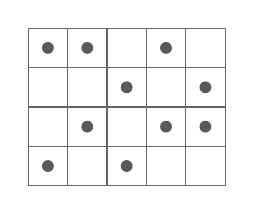
\begin{tikzpicture}[scale=0.50]
  % Grid lines
  \draw[step=1cm, black!60!white] (0,0) grid (5,4);
  % Points
  % \foreach \x/\y in {0.5/0.5, 1.5/1.5, 2.5/2.5, 3.5/3.5, 4.5/1.5, 1.5/3.5, 3.5/1.5, 4.5/2.5, 2.5/0.5, 0.5/3.5} {
  % \fill[red] (\x, \y) circle (0.1);
  \foreach \x/\y/\radius in {0.5/0.5/0.15, 1.5/1.5/0.15, 2.5/2.5/0.15, 3.5/3.5/0.15, 4.5/1.5/0.15, 1.5/3.5/0.15, 3.5/1.5/0.15, 4.5/2.5/0.15, 2.5/0.5/0.15, 0.5/3.5/0.15} {
    \fill[black!65] (\x, \y) circle (\radius);
  }
\end{tikzpicture}
\end{textblock}

\begin{textblock}{140}(10,54)
$\left.
\begin{array}{l}
N = 10 \\
V = 20
\end{array}
\right\}$ \small Macro estados


\only<4->{
\begin{flalign*}
& \ \ W = \binom{20}{10} = \num{184756} &&
\end{flalign*}
}

\end{textblock}
}



\only<2->{
\begin{textblock}{140}(70,18)
\phantom{Gas} \\[0.2cm]

\small Expansión de volumen
\end{textblock}

\begin{textblock}{140}(70,28)
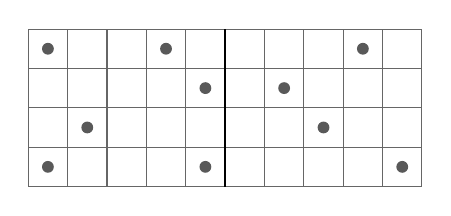
\begin{tikzpicture}[scale=0.50]
  % Grid lines
  \draw[step=1cm, black!60!white] (0,0) grid (10,4);
  % Points
  \foreach \x/\y/\radius in {4.5/0.5/0.15, 0.5/3.5/0.15, 0.5/0.5/0.15, 8.5/3.5/0.15, 4.5/2.5/0.15, 9.5/0.5/0.15, 3.5/3.5/0.15, 1.5/1.5/0.15, 6.5/2.5/0.15,  7.5/1.5/0.15 } {
    \fill[black!65] (\x, \y) circle (\radius);
  }
  % Bold horizontal line
  \draw[line width=1pt] (5,0) -- (5,4);
\end{tikzpicture}
\end{textblock}

\begin{textblock}{140}(70,54)
$\begin{array}{l}
N = 10 \\
V = 40
\end{array}$
\end{textblock}
}


\only<5->{
\begin{textblock}{140}(94,51)
\small
\begin{flalign*}
& W = \binom{40}{10} = \num{847660528} &&
\end{flalign*}
\end{textblock}
}

\only<3>{
\begin{textblock}{160}(0,74)
\centering

¿Cuál es la probabilidad de que se contraiga nuevamente?
\end{textblock}
}

\only<6>{
\begin{textblock}{160}(66,66)
\begin{flalign*}
& P(\text{contraiga}|N=10,V=40) = \frac{\binom{20}{10}}{\binom{40}{10}} = 0.0002 &&
\end{flalign*}
\end{textblock}
}

\end{frame}





\begin{frame}[plain]
\begin{textblock}{160}(0,4)
\centering \LARGE Siglo 19: Física estadística \\
\large Máxima incertidumbre dadas restricciones
\end{textblock}

\only<2->{
\begin{textblock}{130}(10,22)
Restricciones: \normalsize

\hspace{0.3cm} $\bullet$ Partículas totales $N = 6$

\hspace{0.3cm} $\bullet$ Energía total $E = \sum_i e_i \cdot n_i =  6 $


\vspace{0.4cm}

\hspace{-0.7cm}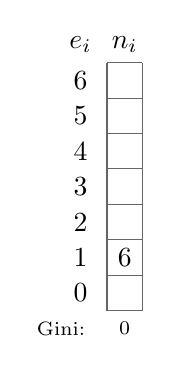
\begin{tikzpicture}[scale=0.45]
  % Grid lines
  \draw[step=1cm, black!60!white] (0,0) grid (1,7);
  % Add character "6" at specified coordinates
  \foreach \x/\y in {-0.75/0.5} {\node at (\x, \y) {0};}
  \foreach \x/\y in {-0.75/1.5} {\node at (\x, \y) {1};}
  \foreach \x/\y in {-0.75/2.5} {\node at (\x, \y) {2};}
  \foreach \x/\y in {-0.75/3.5} {\node at (\x, \y) {3};}
  \foreach \x/\y in {-0.75/4.5} {\node at (\x, \y) {4};}
  \foreach \x/\y in {-0.75/5.5} {\node at (\x, \y) {5};}
  \foreach \x/\y in {-0.75/6.5} {\node at (\x, \y) {6};}
  \foreach \x/\y in {-0.75/7.5} {\node at (\x, \y) {$e_i$};}
  \foreach \x/\y in {0.5/7.5} {\node at (\x, \y) {$n_i$};}
  \onslide<3->{\foreach \x/\y in {0.5/0.5} {\node at (\x, \y) {};}
  \foreach \x/\y in {0.5/1.5} {\node at (\x, \y) {$6$};}
  \foreach \x/\y in {0.5/2.5} {\node at (\x, \y) {};}
  \foreach \x/\y in {0.5/3.5} {\node at (\x, \y) {};}
  \foreach \x/\y in {0.5/4.5} {\node at (\x, \y) {};}
  \foreach \x/\y in {0.5/5.5} {\node at (\x, \y) {};}
  \foreach \x/\y in {0.5/6.5} {\node at (\x, \y) {};}
  }
  \onslide<8->{\foreach \x/\y in {-1.3/-0.5} {\node at (\x, \y) {\scriptsize Gini:};}
  \foreach \x/\y in {0.5/-0.5} {\node at (\x, \y) {\scriptsize $0$};}}
\end{tikzpicture}\hspace{-0.035cm}\onslide<4->{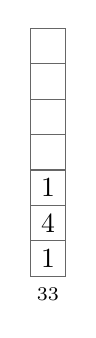
\begin{tikzpicture}[scale=0.45]
  % Grid lines
  \draw[step=1cm, black!60!white] (0,0) grid (1,7);
  % Add character "6" at specified coordinates
  \foreach \x/\y in {0.5/0.5} {\node at (\x, \y) {$1$};}
  \foreach \x/\y in {0.5/1.5} {\node at (\x, \y) {$4$};}
  \foreach \x/\y in {0.5/2.5} {\node at (\x, \y) {$1$};}
  \foreach \x/\y in {0.5/3.5} {\node at (\x, \y) {};}
  \foreach \x/\y in {0.5/4.5} {\node at (\x, \y) {};}
  \foreach \x/\y in {0.5/5.5} {\node at (\x, \y) {};}
  \foreach \x/\y in {0.5/6.5} {\node at (\x, \y) {};}
  \onslide<8->{\phantom{\foreach \x/\y in {0.5/-0.5} {\node at (\x, \y) {\scriptsize G};}}
  \foreach \x/\y in {0.5/-0.5} {\node at (\x, \y) {\scriptsize $33$};}}
\end{tikzpicture}}\onslide<5->{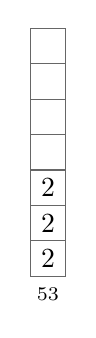
\begin{tikzpicture}[scale=0.45]
  % Grid lines
  \draw[step=1cm, black!60!white] (0,0) grid (1,7);
  % Add character "6" at specified coordinates
  \foreach \x/\y in {0.5/0.5} {\node at (\x, \y) {$2$};}
  \foreach \x/\y in {0.5/1.5} {\node at (\x, \y) {$2$};}
  \foreach \x/\y in {0.5/2.5} {\node at (\x, \y) {$2$};}
  \foreach \x/\y in {0.5/3.5} {\node at (\x, \y) {};}
  \foreach \x/\y in {0.5/4.5} {\node at (\x, \y) {};}
  \foreach \x/\y in {0.5/5.5} {\node at (\x, \y) {};}
  \foreach \x/\y in {0.5/6.5} {\node at (\x, \y) {};}
  \onslide<8->{\phantom{\foreach \x/\y in {0.5/-0.5} {\node at (\x, \y) {\scriptsize G};}}
  \foreach \x/\y in {0.5/-0.5} {\node at (\x, \y) {\scriptsize $53$};}}
\end{tikzpicture}}\onslide<6->{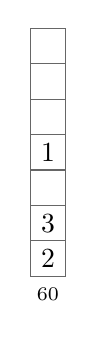
\begin{tikzpicture}[scale=0.45]

  \draw[step=1cm, black!60!white] (0,0) grid (1,7);

  \foreach \x/\y in {0.5/0.5} {\node at (\x, \y) {$2$};}
  \foreach \x/\y in {0.5/1.5} {\node at (\x, \y) {$3$};}
  \foreach \x/\y in {0.5/2.5} {\node at (\x, \y) {};}
  \foreach \x/\y in {0.5/3.5} {\node at (\x, \y) {$1$};}
  \foreach \x/\y in {0.5/4.5} {\node at (\x, \y) {};}
  \foreach \x/\y in {0.5/5.5} {\node at (\x, \y) {};}
  \foreach \x/\y in {0.5/6.5} {\node at (\x, \y) {};}
  \onslide<8->{\phantom{\foreach \x/\y in {0.5/-0.5} {\node at (\x, \y) {\scriptsize G};}}
  \foreach \x/\y in {0.5/-0.5} {\node at (\x, \y) {\scriptsize $60$};}}
\end{tikzpicture}}\onslide<7->{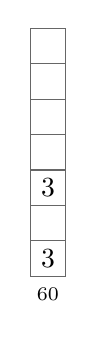
\begin{tikzpicture}[scale=0.45]

  \draw[step=1cm, black!60!white] (0,0) grid (1,7);

  \foreach \x/\y in {0.5/0.5} {\node at (\x, \y) {$3$};}
  \foreach \x/\y in {0.5/1.5} {\node at (\x, \y) {};}
  \foreach \x/\y in {0.5/2.5} {\node at (\x, \y) {$3$};}
  \foreach \x/\y in {0.5/3.5} {\node at (\x, \y) {};}
  \foreach \x/\y in {0.5/4.5} {\node at (\x, \y) {};}
  \foreach \x/\y in {0.5/5.5} {\node at (\x, \y) {};}
  \foreach \x/\y in {0.5/6.5} {\node at (\x, \y) {};}
  \onslide<8->{\phantom{\foreach \x/\y in {0.5/-0.5} {\node at (\x, \y) {\scriptsize G};}}
  \foreach \x/\y in {0.5/-0.5} {\node at (\x, \y) {\scriptsize $60$};}}
\end{tikzpicture}}\onslide<7->{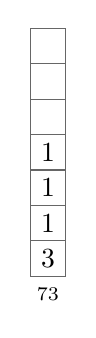
\begin{tikzpicture}[scale=0.45]

  \draw[step=1cm, black!60!white] (0,0) grid (1,7);

  \foreach \x/\y in {0.5/0.5} {\node at (\x, \y) {$3$};}
  \foreach \x/\y in {0.5/1.5} {\node at (\x, \y) {$1$};}
  \foreach \x/\y in {0.5/2.5} {\node at (\x, \y) {$1$};}
  \foreach \x/\y in {0.5/3.5} {\node at (\x, \y) {$1$};}
  \foreach \x/\y in {0.5/4.5} {\node at (\x, \y) {};}
  \foreach \x/\y in {0.5/5.5} {\node at (\x, \y) {};}
  \foreach \x/\y in {0.5/6.5} {\node at (\x, \y) {};}
  \onslide<8->{\phantom{\foreach \x/\y in {0.5/-0.5} {\node at (\x, \y) {\scriptsize G};}}
  \foreach \x/\y in {0.5/-0.5} {\node at (\x, \y) {\scriptsize $73$};}}
\end{tikzpicture}}\onslide<7->{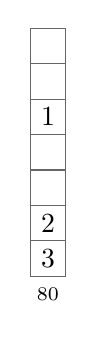
\begin{tikzpicture}[scale=0.45]

  \draw[step=1cm, black!60!white] (0,0) grid (1,7);

  \foreach \x/\y in {0.5/0.5} {\node at (\x, \y) {$3$};}
  \foreach \x/\y in {0.5/1.5} {\node at (\x, \y) {$2$};}
  \foreach \x/\y in {0.5/2.5} {\node at (\x, \y) {};}
  \foreach \x/\y in {0.5/3.5} {\node at (\x, \y) {};}
  \foreach \x/\y in {0.5/4.5} {\node at (\x, \y) {$1$};}
  \foreach \x/\y in {0.5/5.5} {\node at (\x, \y) {};}
  \foreach \x/\y in {0.5/6.5} {\node at (\x, \y) {};}
  \onslide<8->{\phantom{\foreach \x/\y in {0.5/-0.5} {\node at (\x, \y) {\scriptsize G};}}
  \foreach \x/\y in {0.5/-0.5} {\node at (\x, \y) {\scriptsize $80$};}}
\end{tikzpicture}}\onslide<7->{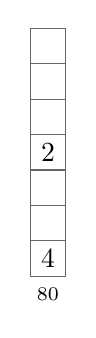
\begin{tikzpicture}[scale=0.45]

  \draw[step=1cm, black!60!white] (0,0) grid (1,7);

  \foreach \x/\y in {0.5/0.5} {\node at (\x, \y) {$4$};}
  \foreach \x/\y in {0.5/1.5} {\node at (\x, \y) {};}
  \foreach \x/\y in {0.5/2.5} {\node at (\x, \y) {};}
  \foreach \x/\y in {0.5/3.5} {\node at (\x, \y) {$2$};}
  \foreach \x/\y in {0.5/4.5} {\node at (\x, \y) {};}
  \foreach \x/\y in {0.5/5.5} {\node at (\x, \y) {};}
  \foreach \x/\y in {0.5/6.5} {\node at (\x, \y) {};}
  \onslide<8->{\phantom{\foreach \x/\y in {0.5/-0.5} {\node at (\x, \y) {\scriptsize G};}}
  \foreach \x/\y in {0.5/-0.5} {\node at (\x, \y) {\scriptsize $80$};}}
\end{tikzpicture}}\onslide<7->{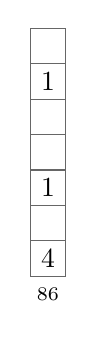
\begin{tikzpicture}[scale=0.45]

  \draw[step=1cm, black!60!white] (0,0) grid (1,7);

  \foreach \x/\y in {0.5/0.5} {\node at (\x, \y) {$4$};}
  \foreach \x/\y in {0.5/1.5} {\node at (\x, \y) {};}
  \foreach \x/\y in {0.5/2.5} {\node at (\x, \y) {$1$};}
  \foreach \x/\y in {0.5/3.5} {\node at (\x, \y) {};}
  \foreach \x/\y in {0.5/4.5} {\node at (\x, \y) {};}
  \foreach \x/\y in {0.5/5.5} {\node at (\x, \y) {$1$};}
  \foreach \x/\y in {0.5/6.5} {\node at (\x, \y) {};}
  \onslide<8->{\phantom{\foreach \x/\y in {0.5/-0.5} {\node at (\x, \y) {\scriptsize G};}}
  \foreach \x/\y in {0.5/-0.5} {\node at (\x, \y) {\scriptsize $86$};}}
\end{tikzpicture}}\onslide<7->{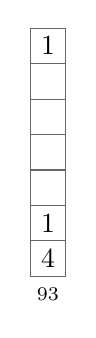
\begin{tikzpicture}[scale=0.45]

  \draw[step=1cm, black!60!white] (0,0) grid (1,7);


  \foreach \x/\y in {0.5/0.5} {\node at (\x, \y) {$4$};}
  \foreach \x/\y in {0.5/1.5} {\node at (\x, \y) {$1$};}
  \foreach \x/\y in {0.5/2.5} {\node at (\x, \y) {};}
  \foreach \x/\y in {0.5/3.5} {\node at (\x, \y) {};}
  \foreach \x/\y in {0.5/4.5} {\node at (\x, \y) {};}
  \foreach \x/\y in {0.5/5.5} {\node at (\x, \y) {};}
  \foreach \x/\y in {0.5/6.5} {\node at (\x, \y) {$1$};}
  \onslide<8->{\phantom{\foreach \x/\y in {0.5/-0.5} {\node at (\x, \y) {\scriptsize G};}}
  \foreach \x/\y in {0.5/-0.5} {\node at (\x, \y) {\scriptsize $93$};}}
\end{tikzpicture}}\hspace{-0.08cm}\onslide<7->{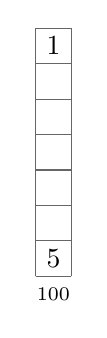
\begin{tikzpicture}[scale=0.45]

  \draw[step=1cm, black!60!white] (0,0) grid (1,7);

  \foreach \x/\y in {0.5/0.5} {\node at (\x, \y) {$5$};}
  \foreach \x/\y in {0.5/1.5} {\node at (\x, \y) {};}
  \foreach \x/\y in {0.5/2.5} {\node at (\x, \y) {};}
  \foreach \x/\y in {0.5/3.5} {\node at (\x, \y) {};}
  \foreach \x/\y in {0.5/4.5} {\node at (\x, \y) {};}
  \foreach \x/\y in {0.5/5.5} {\node at (\x, \y) {};}
  \foreach \x/\y in {0.5/6.5} {\node at (\x, \y) {$1$};}
  \onslide<8->{\phantom{\foreach \x/\y in {0.5/-0.5} {\node at (\x, \y) {\scriptsize G};}}
  \foreach \x/\y in {0.5/-0.5} {\node at (\x, \y) {\scriptsize $100$};}}
\end{tikzpicture}}
\end{textblock}
}

\only<9->{
\begin{textblock}{80}(80,22)
\centering \normalsize
\begin{flalign*}
& W(n_0, n_1, n_2, n_3, n_4, n_5, n_6)  = \frac{N!}{\prod_i n_i !} \\
\only<10-13>{& \ \ W(0, 6, 0, 0, 0, 0, 0)  = 1 \\}
\only<11-13>{& \ \ W(1, 4, 1, 0, 0, 0, 0)  = 30 \\}
\only<12-13>{& \ \ W(2, 2, 2, 0, 0, 0, 0)  = 90 \\}
\only<13>{& \ \ \dots \\}
\only<13>{& \ \ W(5, 0, 0, 0, 0, 0, 1)  = 6 \\}
&&
\end{flalign*}
\end{textblock}
}

\only<14>{
\begin{textblock}{78}(79,42)
\centering
\includegraphics[width=\textwidth, page=1]{figuras/energia.pdf}
\end{textblock}
}


\end{frame}

\begin{frame}[plain]
\begin{textblock}{160}(0,4)
\centering \LARGE Siglo 19: Física estadística \\
\large Entropía
\end{textblock}

%
% \only<3-5>{
% \begin{textblock}{140}(8,26)
% \begin{tikzpicture}[scale=0.50]
% % Draw the surrounding box
%   \draw[red!60, thick] (-0.2, -0.4) rectangle (10.9, 4.4);
% \end{tikzpicture}
% \end{textblock}
% }
%
% \only<-5>{
% \begin{textblock}{140}(10,28)
% \begin{tikzpicture}[scale=0.50]
%   % Grid lines
%   \draw[step=1cm, black!60!white] (0,0) grid (5,4);
%   % Points
%   % \foreach \x/\y in {0.5/0.5, 1.5/1.5, 2.5/2.5, 3.5/3.5, 4.5/1.5, 1.5/3.5, 3.5/1.5, 4.5/2.5, 2.5/0.5, 0.5/3.5} {
%   % \fill[red] (\x, \y) circle (0.1);
%   \foreach \x/\y/\radius in {0.5/0.5/0.15, 1.5/1.5/0.15, 2.5/2.5/0.15, 3.5/3.5/0.15, 4.5/1.5/0.15, 1.5/3.5/0.15, 3.5/1.5/0.15, 4.5/2.5/0.15, 2.5/0.5/0.15, 0.5/3.5/0.15} {
%     \fill[black!65] (\x, \y) circle (\radius);
%   }
% \end{tikzpicture}
% \only<2->{\begin{tikzpicture}[scale=0.50]
%   % Grid lines
%   \draw[step=1cm, black!60!white] (0,0) grid (5,4);
%   % Points
%   % \foreach \x/\y in {0.5/0.5, 1.5/1.5, 2.5/2.5, 3.5/3.5, 4.5/1.5, 1.5/3.5, 3.5/1.5, 4.5/2.5, 2.5/0.5, 0.5/3.5} {
%   % \fill[red] (\x, \y) circle (0.1);
%   \foreach \x/\y/\radius in {1.5/0.5/0.15, 0.5/1.5/0.15, 3.5/2.5/0.15, 3.5/3.5/0.15, 4.5/1.5/0.15, 1.5/3.5/0.15, 3.5/1.5/0.15, 4.5/0.5/0.15, 2.5/1.5/0.15, 0.5/2.5/0.15} {
%     \fill[black!65] (\x, \y) circle (\radius);
%   }
%
% \end{tikzpicture}}
% \end{textblock}
%
% \begin{textblock}{140}(10,54)
% $\begin{array}{l}
% N_A = 10 \\
% V_A = 20
% \end{array}
% $ \small
%
% \begin{flalign*}
% & \ \ W_A = \binom{20}{10} &&
% \end{flalign*}
% \end{textblock}
% }
%
% \only<2-5>{
% \begin{textblock}{140}(40,54)
% $\begin{array}{l}
% N_B = 10 \\
% V_B = 20
% \end{array}
% $ \small
%
% \begin{flalign*}
% & \ \ W_B = \binom{20}{10} &&
% \end{flalign*}
%
% \end{textblock}
% }
%
% \only<4-5>{
% \begin{textblock}{140}(70,24)
% \begin{flalign*}
% N_{AB} &= N_A + N_B \\
% V_{AB} &= V_A + V_B \\
% \only<4>{\phantom}{\log} \, \bm{W_{AB}} &= \bm{W_A} \only<4>{\phantom}{+}  \bm{W_B} \\ &&
% \end{flalign*}
% \end{textblock}
% }

\only<1->{
\begin{textblock}{140}(16,20)
\begin{flalign*}
S = \log W = &
\only<1>{\log \frac{N!}{\prod_i n_i!}}
\only<2->{\log N! - \sum_i \log n_i!}
\phantom{\frac{N!}{\prod_i n_i}} \\
& \only<6-7>{= N \log N - N - \big(\sum_i n_i \log n_i - n_i\big)}
\only<8>{= N \log N - N - \sum_i n_i \log n_i - \sum_i n_i}
\only<9->{= N \log N - \cancel{N} - \sum_i n_i \log n_i + \cancel{\sum_i n_i} } \phantom{\cancel{\sum_i n_i} } \\
& \only<10->{= (\sum_i n_i) \log N - \sum_i n_i \log n_i  } \\
& \only<11>{= \sum_i n_i ( \log N - \log n_i )  }
\only<12>{= \sum_i n_i  \log \frac{N}{n_i}   }
\only<13->{= - \sum_i n_i  \log \frac{n_i}{N}   } \phantom{\frac{N}{n_i} } \\
\only<14>{\frac{S}{N} & = - \sum_i \frac{n_i}{N}  \log \frac{n_i}{N}   }
\only<15->{\frac{S}{N} & = - \sum_i p_i  \log p_i   } \only<16>{= \text{Entropía}}
\phantom{\frac{N}{n_i} }
\\&&
\end{flalign*}
\end{textblock}
}


\only<3-6>{
\begin{textblock}{140}(10,52)
\begin{flalign*}
\log N! = \sum_{k=1}^N \log k & \only<4->{\approx \int_1^N \log k \ dk} \\ \only<5->{&= N \log N - N \cancel{+ 1}} &&
\end{flalign*}
\end{textblock}
}

\only<4>{
\begin{textblock}{70}(80,48)
\includegraphics[width=\textwidth, page=1]{figuras/stirling.pdf}
\end{textblock}
}

\only<5-6>{
\begin{textblock}{70}(80,48)
\includegraphics[width=\textwidth, page=2]{figuras/stirling.pdf}
\end{textblock}
}


\end{frame}


\begin{frame}[plain]
\begin{textblock}{160}(0,4)
\centering  \LARGE Modelo lineal
\end{textblock}


\begin{textblock}{160}(0,18)
\begin{equation*}
\begin{split}
y & = w_0 + w_1 x \\[0.2cm]
p(t | x, \bm{w}, \beta ) &= \N(t \,|\, y(x, \bm{w}), \beta^2) \\[0.6cm]
\onslide<2->{
p(w_i) &= \N(w_i \,|\, 0, \sigma_{i}^2) \\[0cm]}
\end{split}
\end{equation*}
\end{textblock}

\only<3->{
\begin{textblock}{160}(0,54)
\begin{figure}[H]
    \centering
    \tikz{

    \node[latent, fill=black!100, minimum size=2pt] (x) {} ; %
    \node[const, right=of x] (c_x) {$x_i$};
    \node[latent, fill=black!20, yshift=-1.5cm] (t) {$t_i$} ; %
    \node[latent, fill=black!100, yshift=-1.5cm , xshift=-2cm,minimum size=2pt] (beta)
    {} ; %
    \node[const, above=of beta] (c_beta) {$\beta$};
    \node[latent, fill=black!0, yshift=-1.5cm, xshift=2cm] (w) {$\bm{w}$};
    \node[latent, fill=black!100, xshift=2cm, minimum size=2pt] (alpha) {} ; %
    \node[const, right=of alpha] (c_alpha) {$\sigma$};

    \edge {x,beta,w} {t};
    \edge {alpha} {w};

    \node[invisible, fill=black!0, minimum size=0pt, xshift=0.52cm] (data_inv) {} ; %

    \plate {no} {(x)(t)(data_inv)} {$i: $ Datos}; %
    }
\end{figure}
\end{textblock}
}

\end{frame}


\begin{frame}[plain]

\Wider[-3cm]{
 \begin{figure}
\begin{subfigure}[t]{0.32\textwidth}
\onslide<3->{\caption*{Verosimilitud}}
\end{subfigure}
\begin{subfigure}[t]{0.32\textwidth}
\caption*{Priori\onslide<3->{/Posteriori}}
\includegraphics[width=\textwidth]{figuras/pdf/linearRegression_posterior_0.pdf}
\end{subfigure}
\begin{subfigure}[t]{0.32\textwidth}
\onslide<2->{
\caption*{Espacio de datos}
\includegraphics[width=\textwidth]{figuras/pdf/linearRegression_dataSpace_0.pdf}}
\end{subfigure}


\begin{subfigure}[c]{0.32\textwidth}
\onslide<3->{\includegraphics[width=\textwidth]{figuras/pdf/linearRegression_likelihood_1.pdf}}
\end{subfigure}
\begin{subfigure}[c]{0.32\textwidth}
\onslide<3->{\includegraphics[width=\textwidth]{figuras/pdf/linearRegression_posterior_1.pdf}}
\end{subfigure}
\begin{subfigure}[c]{0.32\textwidth}
\onslide<3->{\includegraphics[width=\textwidth]{figuras/pdf/linearRegression_dataSpace_1.pdf}}
\end{subfigure}

\begin{subfigure}[c]{0.32\textwidth}
\onslide<4->{\includegraphics[width=\textwidth]{figuras/pdf/linearRegression_likelihood_2.pdf}}
\end{subfigure}
\begin{subfigure}[c]{0.32\textwidth}
\onslide<4->{\includegraphics[width=\textwidth]{figuras/pdf/linearRegression_posterior_2.pdf}}
\end{subfigure}
\begin{subfigure}[c]{0.32\textwidth}
\onslide<4->{\includegraphics[width=\textwidth]{figuras/pdf/linearRegression_dataSpace_2.pdf}}
\end{subfigure}

\end{figure}
}
\end{frame}



\begin{frame}[plain]
\begin{textblock}{160}(0,4)
\centering \Large Modelos lineales
\end{textblock}
 \vspace{1.25cm}

\only<1->{
\begin{textblock}{80}(0,18)\centering
\ \ Función objetivo \\

$\N(y \,| \, \text{sen}(x), \beta^2) \ \ x \in [-\pi,\pi]$ \\[0.2cm]

       \includegraphics[width=0.85\textwidth]{figuras/pdf/model_selection_true_and_sample}
\end{textblock}
}

\only<2->{
\begin{textblock}{80}(75,22)
\begin{align*}
y &= w_0 + w_1 \, x + w_2 \, x^2 + w_3 \, x^3 \\[1cm]
\onslide<3->{& y  = \sum_{i=0}^{M-1} w_i \phi_i(x) = \bm{w}^T \bm{\phi}(x) \\[0.1cm]
\text{¿}&\text{Cuál es el mejor modelo lineal?}
}
\end{align*}
\end{textblock}
}

\end{frame}



\begin{frame}[plain]
\begin{textblock}{160}(0,4)
\centering \LARGE Siglo 20: Frecuentismo \\
\large \sout{Evaluación} Selección de hipótesis
\end{textblock}


\only<1-10>{
\begin{textblock}{160}(0,14) \centering
\begin{equation*}
 \underset{\bm{w}}{\text{ max }} P(\bm{t} | \bm{x}, \bm{w}, \beta) = \underset{\bm{w}}{\text{ min }} \sum_{i=1}^{n}  (t_i - \bm{w}^T\bm{\phi}(\bm{x}_i))^2
\end{equation*}
\end{textblock}
}


\only<11>{
\begin{textblock}{160}(0,20) \centering
\Large ¿Qué pasa si empezamos a ver datos $x \notin [-\pi,\pi]$?
\end{textblock}
}


\begin{textblock}{80}(0,34)\centering
\only<2-3>{\includegraphics[width=0.9\textwidth]{figuras/pdf/model_selection_OLS.pdf}}\only<4>{\includegraphics[width=0.9\textwidth]{figuras/pdf/model_selection_OLS_best-at-train.pdf}}
\end{textblock}



\only<3-4>{
\begin{textblock}{80}(80,35)\centering
\includegraphics[width=0.9\textwidth]{figuras/pdf/model_selection_maxLikelihood.pdf}
\end{textblock}
}


\only<5-9>{
\begin{textblock}{140}(10,36)\centering
\begin{align*}
P(\text{dato}|\text{Modelo}) & = \only<6->{\phantom}{\sum_{\text{hipótesis}}}  P(\text{dato} \, | \, \text{hipótesis}, \text{Modelo}) \only<6->{\phantom}{P(\text{hipótesis} | \text{Modelo})} \\
\only<7->{& = P(\text{dato} \, | \, \overbrace{\underset{h}{\text{arg max}} \ P(\text{dato}|h, \text{Modelo})}^{\text{Hipótesis que mejor predice}},  \, \text{Modelo} )} \\[0.5cm]
\onslide<9>{P(\text{dato}_{\textbf{Testear}}|\text{Modelo}) & = P(\text{dato}_{\textbf{Testear}} \, | \, \underset{h}{\text{arg max}} \ P(\text{dato}_{\textbf{Entrenar}}|h, \text{Modelo}),  \, \text{Modelo} )}
\end{align*}

\onslide<9>{Testeo y Entrenamiento}

\end{textblock}
}


\only<8>{
\begin{textblock}{140}(10,72)\centering
\Large

¿Predecimos o ``post-decimos''?
\end{textblock}
}



\only<10->{
\begin{textblock}{160}(0,33.5)\centering
\phantom{y} Con testeo y entrenamiento

\includegraphics[width=0.43\textwidth]{figuras/pdf/model_selection_OLS_best-at-test.pdf} \hspace{0.4cm}
\onslide<10->{\includegraphics[width=0.42\textwidth]{figuras/pdf/model_selection_maxApriori_online.pdf}}
\end{textblock}
}


\end{frame}



\begin{frame}[plain]

\centering
\LARGE

¿La aplicación estricta de la probabilidad  \\

produce sobreajuste (\textit{overfitting})?


\end{frame}



\begin{frame}[plain]
\begin{textblock}{160}(0,4)
\centering  \LARGE Siglo 21: Enfoque bayesiano \\
\large Aplicación estricta de las reglas de la probabilidad
\end{textblock}

\begin{textblock}{80}(80,22)\Large
\begin{equation*}
P(\text{Modelo}|\text{Datos})
\end{equation*}
\end{textblock}


\begin{textblock}{160}(0,32)
     \centering
       \includegraphics[width=0.45\textwidth]{figuras/pdf/model_selection_MAP_non-informative}
       \includegraphics[width=0.445\textwidth]{figuras/pdf/model_selection_evidence}
\end{textblock}

\end{frame}


\begin{frame}[plain]
\begin{textblock}{160}(0,4)
\centering \LARGE La función de costo epistémica \\
\end{textblock}


\begin{textblock}{160}(0,22) \centering
\Large Todos los datos son de testeo y entrenamiento:
\large
\begin{equation*}
\underbrace{P(\text{\En{Data}\Es{Datos}} = \{d_1, d_2, \dots \}|\text{Modelo})}_{\text{\small Evidencia: predicción del modelo}}  =  \underbrace{P(d_1 |\text{Modelo})}_{\text{\small Predic\En{tion}\Es{ción} 1}} \, \underbrace{P(d_2 | d_1 , \text{Modelo})}_{\text{\small Predic\En{tion}\Es{ción} 2}} \dots
\end{equation*}
\end{textblock}

\only<2->{
\begin{textblock}{140}(10,56)\centering
\Large La predicción se hace con todas las hipótesis \large
\begin{align*}
P(\text{dato}_1|\text{Modelo}) & = \sum_{\text{hipótesis}}  P(\text{dato}_1| \text{hipótesis}, \text{Modelo}) P(\text{hipótesis} | \text{Modelo}) \\[0.2cm]
%\onslide<3>{P(\text{Datos}) & = \sum_{\text{Modelo}} P(\text{Datos}\,| \text{Modelo}) \, P(\text{Modelo})}
\end{align*}
\end{textblock}
}


\end{frame}


\begin{frame}[plain]
\begin{textblock}{160}(0,4)
\centering \LARGE  Evidencia \\
\large Balance natural entre complejidad y predicci\'on
\end{textblock}


 \begin{textblock}{120}(20,12)
  \centering
  \includegraphics[width=0.9\textwidth]{figuras/pdf/evidencia_de_modelos_alternativos}
 \end{textblock}

  \end{frame}



\begin{frame}[plain]
\begin{textblock}{160}(0,4)
\centering \LARGE  La verdadera predicción \\
\large Predicción con la contribución de todos los modelos
\end{textblock}


\begin{textblock}{160}(0,21)
\begin{equation*}
P(\text{Datos}) =  \sum_{\text{Modelo}} P(\text{Datos}|\text{Modelo}) P(\text{Modelo})
\end{equation*}
\end{textblock}

%
% \begin{textblock}{160}(0,35)\large
% \begin{equation*}
% P(\text{Modelo}|\text{Datos})
% \end{equation*}
% \end{textblock}


\only<2>{
\begin{textblock}{70}(5,50)
     \centering

     Si aparecen datos $x \notin [-\pi, \pi]$ van a poder ser explicados con los modelos más complejos
\end{textblock}


\begin{textblock}{80}(80,40)
     \centering
       \includegraphics[width=0.8\textwidth]{figuras/pdf/model_selection_evidence} \hfill
\end{textblock}
}

\end{frame}






%
% \begin{frame}[plain]
% \begin{textblock}{140}(10,28)
% \Large Ejercicio 1.1 \\[0.4cm]
%
% \large La persona que da la pista a veces se confunde y señala la caja donde está el regalo o la caja que fue elegida previamente por la persona. \\[0.2cm]
%
% \only<2>{
% \large Descubrir el verdadero efecto causal que el regalo y la elección tienen sobre la pista en base a los datos ofrecidos en la práctica. \\[0.1cm]}
%
% \end{textblock}
%
%
% \end{frame}

\begin{frame}[plain,noframenumbering]
\centering \vspace{0.5cm}
\includegraphics[width=1\textwidth]{../../auxiliar/static/BP.png}
\end{frame}





%
% \begin{frame}[plain]
% \begin{textblock}{96}(0,6.5)\centering
% {\transparent{0.9}\includegraphics[width=0.8\textwidth]{../../auxiliar/static/inti.png}}
% \end{textblock}
%
% \begin{textblock}{160}(96,5.5)
% \includegraphics[width=0.35\textwidth]{../../auxiliar/static/pachacuteckoricancha}
% \end{textblock}
% \end{frame}





\end{document}



